%\documentclass[letterpaper,12pt]{article}
\documentclass{mcp}

\usepackage{graphics}

\usepackage{geometry}
%\usepackage{amsmath}
%\usepackage{amsfonts}
\usepackage{amssymb}
\usepackage{bm}
\usepackage{algorithmic}
\usepackage{algorithm}
\usepackage{rotating}
\usepackage[caption=false,font=footnotesize]{subfig}
\usepackage{color}
\usepackage{tikz}
\usetikzlibrary{shapes,arrows,backgrounds,calc,positioning,fit,petri,plotmarks}
\usepackage{multirow}
\usepackage{graphicx}
\usepackage{subfig}
\usepackage{url}
\usepackage{booktabs}
\usepackage{enumitem}
\usepackage{authblk}


\def\todo#1{{\color{red}[TODO: #1]}}


%\usepackage{caption} 
%\captionsetup[table]{skip=10pt}
\captionsetup{belowskip=12pt,aboveskip=4pt}

% strikkeout \sout
\usepackage[normalem]{ulem}


\usepackage{fullpage}
\usepackage{amsfonts,amsthm}
\usepackage{amsmath}
%\usepackage[fleqn]{amsmath}
%\usepackage{setspace}
%\usepackage{url}

%\usepackage[table,dvipsnames]{xcolor}
%\usepackage{textcomp}
%\usepackage{gensymb}

\usepackage{fancyhdr}
\pagestyle{fancy}
\lhead{\footnotesize \parbox{11cm}{Supplementary }}
\headsep = 25pt

%\usepackage{tabulary,multirow,multicol,rotating}

%% big wide hat
\usepackage{scalerel,stackengine}
\stackMath
\newcommand\reallywidehat[1]{%
\savestack{\tmpbox}{\stretchto{%
  \scaleto{%
    \scalerel*[\widthof{\ensuremath{#1}}]{\kern-.6pt\bigwedge\kern-.6pt}%
    {\rule[-\textheight/2]{1ex}{\textheight}}%WIDTH-LIMITED BIG WEDGE
  }{\textheight}% 
}{0.5ex}}%
\stackon[1pt]{#1}{\tmpbox}%
}
\parskip 1ex

\renewcommand{\thetable}{S\arabic{table}}
\renewcommand{\thefigure}{S\arabic{figure}}
%\renewcommand{\tablename}{Supplementary Table}
%\renewcommand{\figurename}{Supplementary Figure}

\def\sfigref#1{{Figure~\ref{#1}}}
\def\secref#1{Section~\ref{#1}}
\def\stabref#1{{Table~\ref{#1}}}
\def\seqref#1{Eq.~(\ref{#1})}

%\floatname{algorithm}{Procedure}
%\renewcommand{\algorithmicrequire}{\textbf{Input:}}
%\renewcommand{\algorithmicensure}{\textbf{Output:}}


\title{Statistical methods for relative quantification of post-translational modifications in global proteomics experiments}
\author[1]{Tsung-Heng~Tsai}
%\author[1]{Olga~Vitek}
\affil[1]{Northeastern University, Boston, MA, USA}


\begin{document}
%\maketitle

%\newpage
%\tableofcontents


%%%%%%%%%%%%%%%%%%%%%%%%%%%%%%%%%%%%%%%%%%%%%%%%%%%%%%%%%%%%%%%%
\section{The motivating example}
\label{sec:motiv}

\todo{use a more representative plot}

\todo{change the order of the panels, so that the modified and unmodified peptides are in the first row, the modified peptides without a counterpart are in the second row left column (right column empty), and the unmodified peptides without a counterpart are in the third row right column (left column empty)}

\todo{the batches are not very clear from the plot}

\begin{figure}[h!]
\centering
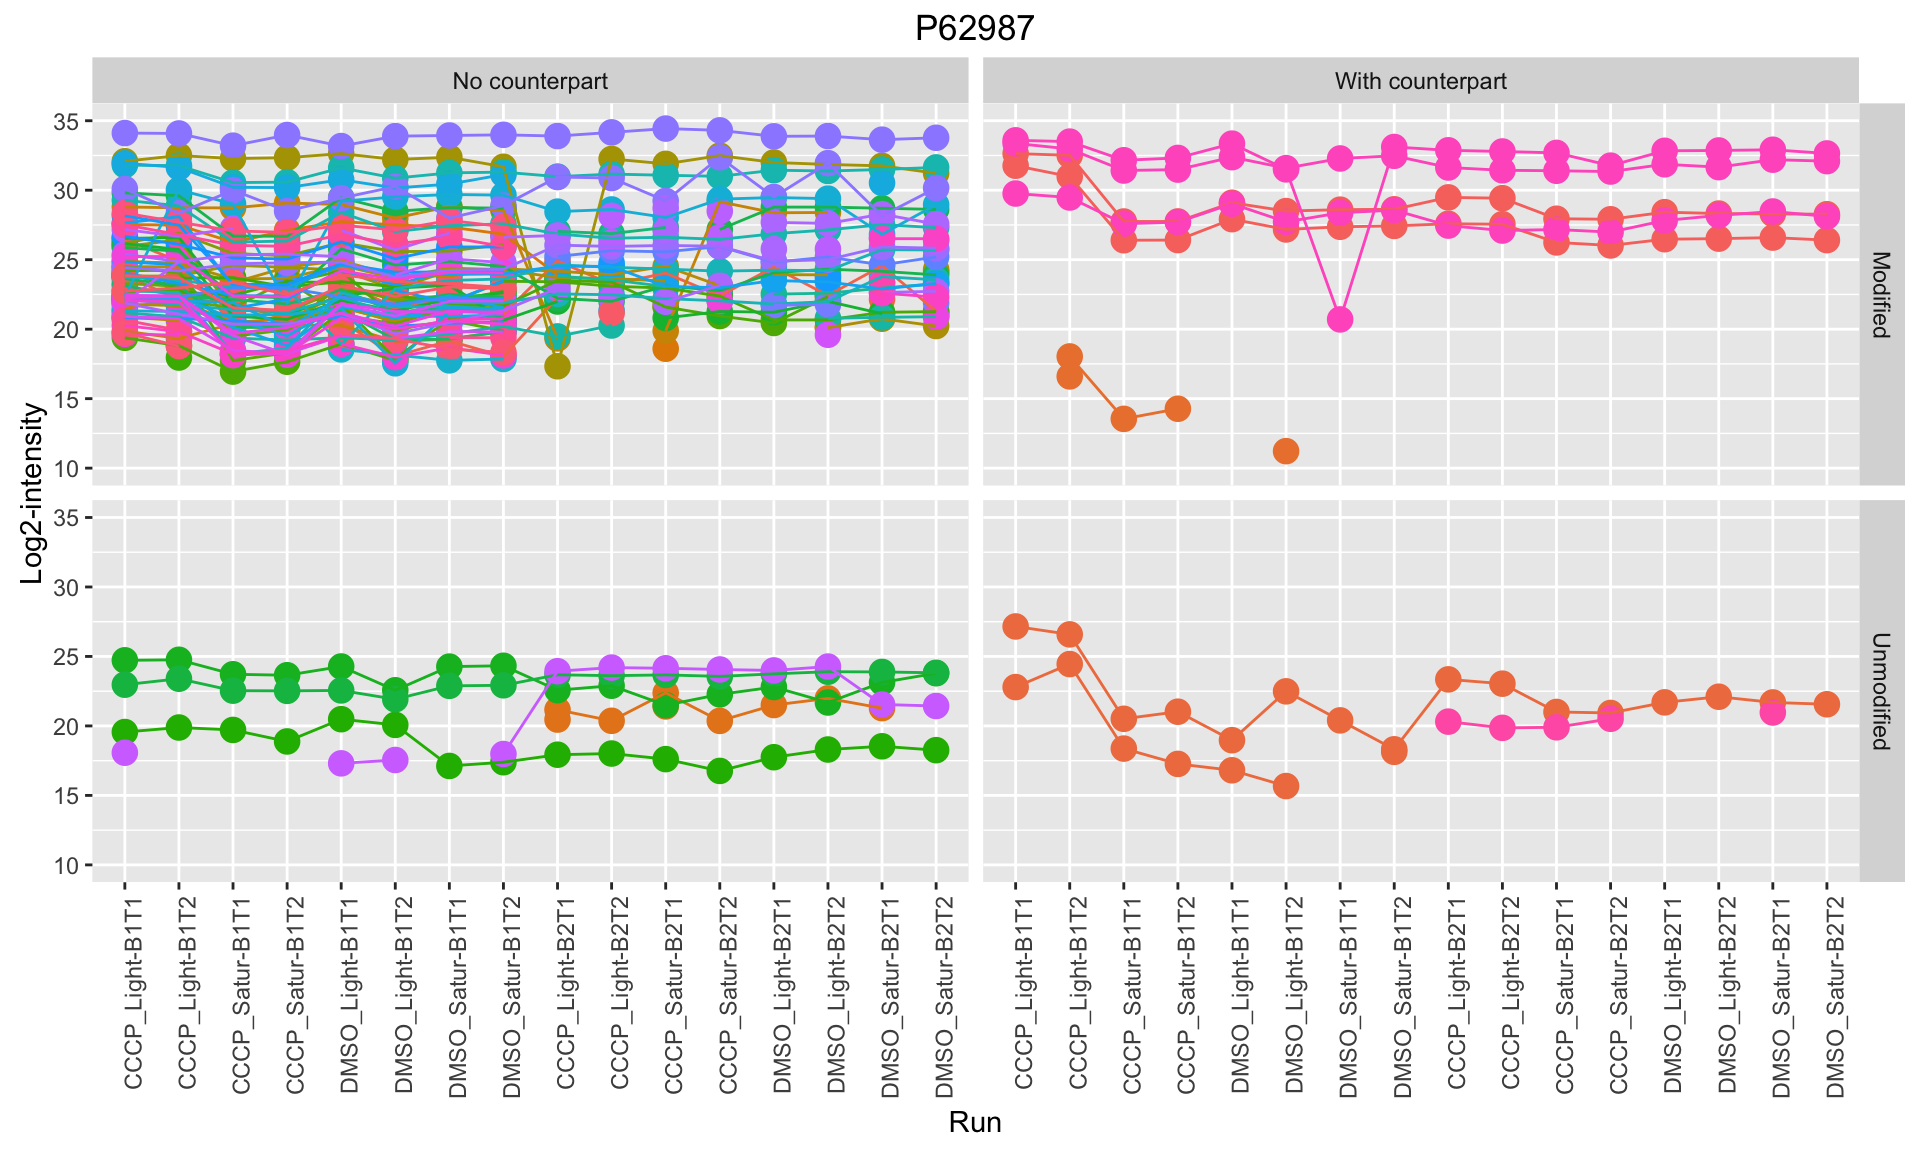
\includegraphics[width=.9\textwidth]{fig/ex_profile}
\caption{Profile plot of peptide features categorized based on modification and matching status.}
\end{figure}

In a typical PTM experiment, modified and unmodified forms of the same peptide can have very different quantitative characteristics such as ionization efficiency and associated variability. Observed changes in signal intensities of modified peptides may result from changes in modification as well as changes in protein abundance. To account for this confounding factor, unmodified peptides that do not contain any modified sites are used for estimation of the underlying protein abundance. Data are often acquired in multiple batches, which is another factor affecting the quantitative characteristics. As shown in the profile plot, the number of peptide features and their intensities vary across batches. 


%%%%%%%%%%%%%%%%%%%%%%%%%%%%%%%%%%%%%%%%%%%%%%%%%%%%%%%%%%%%%%%%
\clearpage
\section{Overview of proposed approach and notation}
\label{sec:intro}

\todo{Make it more clear that this data structure reflects a particular site. Mention somewhere that we only consider peptides with one modifiable site}

\todo{The definition of a batch is not very clear. Can you define it in a way that is not very specific to these particular experiments?}

\todo{Why do you need stars in this table? Maybe simplify and say that this table is for unmodified peptides, and that a similar table is constructed for the modified peptides, with y*?}

The main objective is to detect modifications that are differentially expressed across experimental conditions.

%Unlike protein-level analysis, in which multiple quantified peptides are often observed, phospho-peptides are more frequently detected and quantified only once. There is a strong correlation between signal strength and reproducibility. When selecting sites for further study, investigators should pay close attention to the number of PSMs and the signal strength for peptides harboring each site.
%Simply calculating averages or medians of all peptides containing a given site might not reval the full complexity of cellular phosphorylation patterns. Singly and doubly phosphorylated forms of a peptide might be present at different levels. One must also not forget taht changes in total protein level are not refelcted in the phosphopeptide ratios. Whenever possible, separate protein-level measurements made from unmodified peptides should be performed and used to normalize phosphopeptide ratios.


\paragraph{Data structure of PTM quantification experiments.}
A set of fully-cleaved and/or partially-cleaved peptides with a same modification (e.g., ubiquitination) at one site are considered together. There are $I$ conditions and $J$ mass spectrometry runs (technical replicates) per condition, processed in $B$ batches in the experiment. In each batch, there are $K \times L$ runs. 
The modification is represented by multiple spectral features (peptide ions, distinguished by their cleavage sites, mass shifts and charge states), where the number of features in Batch $b$ is $K_b$. The log-intensity (base 2) of Feature $k$, in Run $j$ of Condition $i$ in Batch $b$ is denoted by $y_{b,ijk}^{\ast}$. 

\begin{figure}[h!]
\centering
\begin{footnotesize}
\[
\begin{array}{l l c c c c c c c c c} 
\toprule
 &  & \multicolumn{4}{c}{\text{Condition }1} & \dots & \multicolumn{4}{c}{\text{Condition }I} \\ 
\cmidrule{3-6} 
\cmidrule{8-11} 
 &  &  \text{Run }1 & \text{Run }2 & \dots & \text{Run }J & \dots & \text{Run }1 & \text{Run }2 & \dots & \text{Run }J \\
\midrule
\multirow{4}{*}{Batch $1$} & \text{Feature }1 & y_{1,111}^{\ast} & y_{1,121}^{\ast} & \dots & y_{1,1J1}^{\ast} & \dots & y_{1,I11}^{\ast} & y_{1,I21}^{\ast} & \dots & y_{1,IJ1}^{\ast} \\
 & \text{Feature }2 & y_{1,112}^{\ast} & y_{1,122}^{\ast} & \dots & y_{1,1J2}^{\ast} & \dots & y_{1,I12}^{\ast} & y_{1,I22}^{\ast} & \dots & y_{1,IJ2}^{\ast}  \\
 & \dots & \dots & \dots & \dots & \dots & \dots & \dots & \dots & \dots & \dots \\
 & \text{Feature }K_1 & y_{1,11K_1}^{\ast} & y_{1,12K_1}^{\ast} & \dots & y_{1,1JK_1}^{\ast} & \dots & y_{1,I1K_1}^{\ast} & y_{1,I2K_1}^{\ast} & \dots & y_{1,IJK_1}^{\ast} \\
\midrule
\dots & \dots & \dots & \dots & \dots & \dots & \dots & \dots & \dots & \dots & \dots \\
\dots & \dots & \dots & \dots & \dots & \dots & \dots & \dots & \dots & \dots & \dots \\
\midrule
\multirow{4}{*}{Batch $b$} & \text{Feature }1 & y_{b,111}^{\ast} & y_{b,121}^{\ast} & \dots & y_{b,1J1}^{\ast} & \dots & y_{b,I11}^{\ast} & y_{b,I21}^{\ast} & \dots & y_{b,IJ1}^{\ast} \\
 & \text{Feature }2 & y_{b,112}^{\ast} & y_{b,122}^{\ast} & \dots & y_{b,1J2}^{\ast} & \dots & y_{b,I12}^{\ast} & y_{b,I22}^{\ast} & \dots & y_{b,IJ2}^{\ast}  \\
 & \dots & \dots & \dots & \dots & \dots & \dots & \dots & \dots & \dots & \dots \\
 & \text{Feature }K_b & y_{b,11K_b}^{\ast} & y_{b,12K_b}^{\ast} & \dots & y_{b,1JK_b}^{\ast} & \dots & y_{b,I1K_b}^{\ast} & y_{b,I2K_b}^{\ast} & \dots & y_{b,IJK_b}^{\ast} \\
\midrule
\dots & \dots & \dots & \dots & \dots & \dots & \dots & \dots & \dots & \dots & \dots \\
\dots & \dots & \dots & \dots & \dots & \dots & \dots & \dots & \dots & \dots & \dots \\
\midrule
\multirow{4}{*}{Batch $B$} & \text{Feature }1 & y_{B,111}^{\ast} & y_{B,121}^{\ast} & \dots & y_{B,1J1}^{\ast} & \dots & y_{B,I11}^{\ast} & y_{B,I21}^{\ast} & \dots & y_{B,IJ1}^{\ast} \\
 & \text{Feature }2 & y_{B,112}^{\ast} & y_{B,122}^{\ast} & \dots & y_{B,1J2}^{\ast} & \dots & y_{B,I12}^{\ast} & y_{B,I22}^{\ast} & \dots & y_{B,IJ2}^{\ast}  \\
 & \dots & \dots & \dots & \dots & \dots & \dots & \dots & \dots & \dots & \dots \\
 & \text{Feature }K_B & y_{B,11K_B}^{\ast} & y_{B,12K_B}^{\ast} & \dots & y_{B,1JK_B}^{\ast} & \dots & y_{B,I1K_B}^{\ast} & y_{B,I2K_B}^{\ast} & \dots & y_{B,IJK_B}^{\ast} \\
%\midrule
%\multirow{4}{*}{\text{Batch }1} & \text{Feature }1 & y_{b,111} & y_{b,121} & \dots & y_{b,1J1} & \dots & y_{b,I11} & y_{b,I21} & \dots & y_{b,IJ1} \\
% & \text{Feature }2 & y_{b,112} & y_{b,122} & \dots & y_{b,1J2} & \dots & y_{b,I12} & y_{b,I22} & \dots & y_{b,IJ2}  \\
% & \dots & \dots & \dots & \dots & \dots & \dots & \dots & \dots & \dots & \dots \\
% & \text{Feature }L & y_{b,11L} & y_{b,12L} & \dots & y_{b,1JL} & \dots & y_{b,I1L} & y_{b,I2L} & \dots & y_{b,IJL} \\
\bottomrule
\end{array}
\]
\end{footnotesize}
\caption{Representation of the data of modified peptides at one site, measured in $B$ batches with $I$ conditions and $J$ replicate runs. Modification level is quantified by multiple spectral features (peptide ions). Some spectral features can be missing (shown as $-$), either randomly in individual runs or completely from a particular form. In real practice, the number of runs can vary across conditions. \label{fig:dtable}}
\end{figure}

\sfigref{fig:dtable} shows an example data representation of modified peptide ions at one site. The modification measured in multiple batches is represented by different numbers of features. Unmodified peptides from the same protein are sometimes also measured, which may provide additional evidence on the underlying protein abundance. The features of unmodified peptides are denoted similarly. That is, the log-intensity (base 2) of Feature $l$, in Run $j$ of Condition $i$ in Batch $b$ is denoted by $y_{b,ijl}$, where $l \in \{1, \ldots , L_b \}$. To address the goal, statistical analysis needs to summarize values in this table using appropriate statistical models, translate the goal into a model-based quantity of interest, and draw inference (i.e., characterize the uncertainty) about the quantity. 


%%%%%%%%%%%%%%%%%%%%%%%%%%%%%%%%%%%%%%%%%%%%%%%%%%%%%%%%%%%%%%%%
\section{Existing method: two-sample $t$-test}
\label{sec:ttest}

Two-sample $t$-test is based on the null hypothesis stating that there is no difference in mean modification abundance between Conditions $i$ and $i'$ against the alternative: 
\begin{align*}
H_{0}: \mu_{i}^{\ast} - \mu_{i'}^{\ast} &= 0\\
H_{a}: \mu_{i}^{\ast} - \mu_{i'}^{\ast} &\neq 0
\end{align*}
The test is not directly applicable to a problem with batches of data. Several \textit{ad-hoc} approaches may be used. Three commonly used approaches are 1) $t$-test (no batch): ignoring batch effects when applying $t$-test, 2) $t$-test (most significant batch): applying $t$-test in each batch and drawing conclusions based on the most significant batch, and 3) $t$-test (all batch): applying $t$-test in each batch and drawing conclusions based on all batches. Although simple, these \textit{ad-hoc} methods lack statistical justification. We reconstruct their meanings below and characterize their statistical properties under various forms of batch effects in \secref{sec:sim}. The abundance in each run is taken as input each of the three methods and is often estimated by sum of peak intensities, e.g., the abundance estimate for Run $j$ of Condition $i$ in Batch $b$ is given by
\[
y_{b, ij+} = \sum_{k=1}^{K_b} y_{b, ijk}
\]

%In our implementation of the approach using all batches, estimation of a change is the average over all batches and the readout for statistical significance (i.e., $p$-value) is based on the least significant batch. 


\paragraph{Two-sample $t$-test (no batch).}
In this approach, the modification abundance is estimated as the average over runs in all batches. For example, the estimate for Group $i$ is given by
\[
\hat{\mu}_{i}^{\ast} = \frac{1}{BJ} \sum_{b=1}^{B} \sum_{j=1}^{J} y_{b, ij+}.
\]
This is equivalent to fitting a linear model with only an intercept, which does not account for different characteristics across batches. 


\paragraph{Two-sample $t$-test (most significant batch).} 
The modification abundance is estimated in all batches, i.e., 
\[
\hat{\mu}_{b, i}^{\ast} = \frac{1}{J} \sum_{j=1}^{J} y_{b, ij+},
\]
where $\mathrm{SE} (\hat{\mu}_{b, i}^{\ast})$ is the standard error associated with the estimate. 
The test statistic in Batch $b$ is 
\[
t_{b} = \frac{\hat{\mu}_{b, i}^{\ast}}{\mathrm{SE} (\hat{\mu}_{b, i}^{\ast})}
\]
To summarize the evidence across batches, one strategy is to use the most significant batch. With balanced design, the batch with the largest test statistic across all batch is selected, i.e., 
\[
b_{\text{max}} = \{ b \mid t_b = \max_{b'=1, \ldots, B} | t_{b'} | \}.
\] 
The change in modification abundance is estimated as
\[
\hat{\mu}_{i}^{\ast} - \hat{\mu}_{i'}^{\ast} = \hat{\mu}_{b_{\text{max}}, i}^{\ast} - \hat{\mu}_{b_{\text{max}}, i'}^{\ast}
\]
and the test statistic for the $t$-test is given by
\[
\frac{\hat{\mu}_{i}^{\ast} - \hat{\mu}_{i'}^{\ast}}{\mathrm{SE}\left( \hat{\mu}_{i}^{\ast} - \hat{\mu}_{i'}^{\ast} \right)} 
= \frac{ \hat{\mu}_{b_{\text{max}}, i}^{\ast} - \hat{\mu}_{b_{\text{max}}, i'}^{\ast} }{\left[ \mathrm{SE}(\hat{\mu}_{b_{\text{max}}, i}^{\ast})^2 + \mathrm{SE}(\hat{\mu}_{b_{\text{max}}, i'}^{\ast})^2 \right]^{1/2}},
\]
%where $\hat{\sigma}_{\pi, ijk}^{2}$ and $\hat{\sigma}_{\pi, ijk'}^{2}$ are estimated as sample variances. 


\paragraph{Two-sample $t$-test (all batch).}
A change in modification abundance is considered as statistically significant only if such change is significant in all batches. This is equivalent to take the smallest test statistic across batches for the $t$-test: 
\[
\frac{\hat{\mu}_{i}^{\ast} - \hat{\mu}_{i'}^{\ast}}{\mathrm{SE}\left( \hat{\mu}_{i}^{\ast} - \hat{\mu}_{i'}^{\ast} \right)} 
= \frac{ \hat{\mu}_{b_{\text{min}}, i}^{\ast} - \hat{\mu}_{b_{\text{min}}, i'}^{\ast} }{\left[ \mathrm{SE}(\hat{\mu}_{b_{\text{min}}, i}^{\ast})^2 + \mathrm{SE}(\hat{\mu}_{b_{\text{min}}, i'}^{\ast})^2 \right]^{1/2}},
\]
where 
\[
b_{\text{min}} = \{ b \mid t_b = \min_{b'=1, \ldots, B} | t_{b'} | \}.
\] 



%%%%%%%%%%%%%%%%%%%%%%%%%%%%%%%%%%%%%%%%%%%%%%%%%%%%%%%%%%%%%%%%
\section{Proposed statistical modeling and inference}

To characterize the observed feature intensities, different levels of variations are expressed in consideration of the following factors: modification, batch, condition, run, and feature. As the number of peptide features and their intensities are different across batches, variances of feature intensities are therefore expected to vary across batches. Also, different degrees of variability in the intensities of modified and unmodified features are present in the data; therefore, they are expressed by separate models.

\todo{identify and present the best model that we advocate for}


%%%%%%%%%%%%%%%%%%%%%%%%%%%%%%%%%%%%%%%%%%%%%%%%%%%%%%%%%%%%%%%%
\subsection{Linear models and parameter estimation}

The observed log-intensity of a modified peptide feature in batch $b$ is denoted by $y_{b,ijk}^{\ast}$ and represented as
\[
y_{b,ijk}^{\ast} = \psi_{b}^{\ast} + C_{b,i}^{\ast} + R_{b,j(i)}^{\ast} + F_{b,k}^{\ast} + (R \times F)_{b,ijk}^{\ast},
\]
where the effects of condition and feature are modeled as fixed effects: 
\[
\sum_{i=1}^{I} C_{b,i}^{\ast} = 0, \quad \sum_{k=1}^{K_b} F_{b,k}^{\ast} = 0,
\]
and the effects of run and its interaction with feature are considered as random effects arising from normal distribution with mean $0$: 
\[
R_{b,j(i)}^{\ast} = \gamma_{b,j(i)}^{\ast} \stackrel{\text{iid}}{\sim} \mathcal{N}(0, \sigma_{\gamma_b^{\ast}}^{2}), \qquad
(R \times F)_{b,ijk}^{\ast} = \epsilon_{b,ijk}^{\ast} \stackrel{\text{iid}}{\sim} \mathcal{N}(0, \sigma_{\epsilon_b^{\ast}}^{2}).
\]
Similarly, the observed log-intensity of an unmodified peptide feature is denoted by $y_{b,ijk}$ and represented as 
\[
y_{b,ijl} = \psi_{b} + C_{b,i} + R_{b,j(i)} + F_{b,l} + (R \times F)_{b,ijl}, 
\]
where the effects of condition and feature are modeled as fixed effects: 
\[
\sum_{i=1}^{I} C_{b,i} = 0, \quad \sum_{l=1}^{L_b} F_{b,l} = 0,
\]
and 
\[
R_{b,j(i)} = \gamma_{b,j(i)} \stackrel{\text{iid}}{\sim} \mathcal{N}(0, \sigma_{\gamma_b}^{2}), \qquad
(R \times F)_{b,ijl} = \epsilon_{b,ijl} \stackrel{\text{iid}}{\sim} \mathcal{N}(0, \sigma_{\epsilon_b}^{2}).
\]


%%%%%%%%%%%%%%%%%%%%%%%%%%%%%%%%%%%%%%%%%%%%%%%%%%%%%%%%%%%%%%%%
\subsubsection{Run-level summarization of feature intensities}

The summarization of feature intensities at each site is carried out as in the sub-plot model of MSstats, which involves
\begin{enumerate}
\item Imputation of censored missing values
\item Summarization of feature intensities using Tukey's median polish (TMP), where the summarized log-intensity is denoted by $\hat{y}_{b, ij}$
\end{enumerate}


%%%%%%%%%%%%%%%%%%%%%%%%%%%%%%%%%%%%%%%%%%%%%%%%%%%%%%%%%%%%%%%%
\subsubsection{Model-based inference of the underlying abundance}

We distinguish two candidate models accounting for batch effects: 1) \emph{per-batch model}, which assumes changes between conditions and variability in the run-level summaries are not identical across batches, and each batch needs to be modeled separately, and 2) \emph{all-batch model}, which assumes differences between conditions are consistent across batches (i.e., no interaction effect between condition and batch) and identical variability in the run-level summarization is shared across batches. The details for each model are given below, with a summary in Table XX.

\paragraph{Per-batch model.}
Within Batch $b$, the abundance of the modification in each run is represented as 
\[
\hat{y}_{b, ij}^{\ast} = \psi_{b}^{\ast} + C_{b, i}^{\ast} + R_{b, j(i)}^{\ast},
\]
where $\sum_{i=1}^{I} C_{b, i}^{\ast} = 0$, $R_{b, j(i)}^{\ast} = \gamma_{b, j(i)}^{\ast} \stackrel{\text{iid}}{\sim} \mathcal{N}(0, \sigma_{\gamma_{b}^{\ast}}^{2})$.
Similarly, the model for protein abundance in each run is given by
\[
\hat{y}_{b, ij} = \psi_{b} + C_{b, i} + R_{b, j(i)},
\]
where $\sum_{i=1}^{I} C_{b, i} = 0$, $R_{b, j(i)} = \gamma_{b, j(i)} \stackrel{\text{iid}}{\sim} \mathcal{N}(0, \sigma_{\gamma_{b}}^{2})$. The expected values of log-abundances of the modification and protein in group $i$ are denoted by $\mu_{i}^{\ast}$ and $\mu_{i}$, respectively, and the values are defined as the average over the estimates in all batches:
\begin{align*}
\mu_{i}^{\ast} &= \psi^{\ast} + C_{i}^{\ast} = \frac{1}{B} \sum_{b=1}^{B} (\psi_{b}^{\ast} + C_{b, i}^{\ast})\\
\mu_{i} &= \psi + C_{i} = \frac{1}{B} \sum_{b=1}^{B} (\psi_{b} + C_{b, i})
%\mu_{i} &= \psi + C_{i}.
\end{align*}

\paragraph{All-batch model.} The whole-plot model for the modification abundance in each run is represented as 
\[
\hat{y}_{b, ij}^{\ast} = \psi^{\ast} + \delta_{b}^{\ast} + C_{i}^{\ast} + R_{b, j(i)}^{\ast},
\]
where $\sum_{b=1}^{B} \delta_{b}^{\ast} = 0$, $\sum_{i=1}^{I} C_{i}^{\ast} = 0$, $R_{b, j(i)}^{\ast} = \gamma_{b, j(i)}^{\ast} \stackrel{\text{iid}}{\sim} \mathcal{N}(0, \sigma_{\gamma^{\ast}}^{2})$.
Similarly, the model for protein abundance in each run is given by
\[
\hat{y}_{b, ij} = \psi + \delta_{b} + C_{i} + R_{b, j(i)},
\]
where $\sum_{b=1}^{B} \delta_{b} = 0$, $\sum_{i=1}^{I} C_{i} = 0$, $R_{b, j(i)} = \gamma_{b, j(i)} \stackrel{\text{iid}}{\sim} \mathcal{N}(0, \sigma_{\gamma}^{2})$. The expected values of log-abundances of the modification and protein in group $i$ are defined as $\mu_{i}^{\ast}$ and $\mu_{i}$, respectively. The values are represented as follows
\begin{align*}
\mu_{i}^{\ast} &= \psi^{\ast} + C_{i}^{\ast}\\
\mu_{i} &= \psi + C_{i}
\end{align*}


%%%%%%%%%%%%%%%%%%%%%%%%%%%%%%%%%%%%%%%%%%%%%%%%%%%%%%%%%%%%%%%%
\subsection{Model-based testing}
Hypothesis testing on the log-abundances of the modifications in Conditions $i$ and $i'$ is performed to detect systematic changes in modification abundance. The hypothesis states that there is no difference in log-abundance of the modification between groups $i$ and $i'$
\begin{align*}
H_{0}: \Delta = \mu_{i}^{\ast} - \mu_{i'}^{\ast} &= 0 \\
H_{a}: \Delta = \mu_{i}^{\ast} - \mu_{i'}^{\ast} &\neq 0
\end{align*}
The difference in modification abundance, $\Delta = \mu_{i}^{\ast} - \mu_{i'}^{\ast}$, is estimated with the per-batch model and all-batch model as follows.

\paragraph{Per-batch model.} 
The log of fold change in modification abundance is estimated as the average over batches
\[
\hat{\Delta} = \frac{1}{B} \sum_{b=1}^{B} \left[ \frac{1}{J} \left( \hat{y}_{b,i+}^{\ast} - \hat{y}_{b,i'+}^{\ast} \right) \right],
\]
and the standard error of the estimate is 
\[
\mathrm{SE}(\hat{\Delta}) = \left[ \left(\frac{1}{B}\right)^2 \cdot \frac{2}{J} \sum_{b=1}^{B} \hat{\sigma}_{\gamma_b^{\ast}}^{2} \right]^{1/2}
\]
The test statistic $\hat{\Delta} / \mathrm{SE}(\hat{\Delta})$ is compared against the $t$ distribution. The degrees of freedom of the $t$ distribution are approximated as
%\[
%\frac{ \left( \sum_{b=1}^{B} \hat{\sigma}_{\gamma_{b}^{\ast}}^{2} \right)^2 }
%{ \sum_{b=1}^{B} \left[  \frac{\hat{\sigma}_{\gamma_{b}^{\ast}}^{4}}{ \mathrm{df}(\gamma_b^{\ast}) }  \right] }.
%\]
\[
\left( \sum_{b=1}^{B} \hat{\sigma}_{\gamma_{b}^{\ast}}^{2} \right)^2 \bigg/
\sum_{b=1}^{B} \left[  \frac{\hat{\sigma}_{\gamma_{b}^{\ast}}^{4}}{ \mathrm{df}(\gamma_b^{\ast}) } \right].
\]


\paragraph{All-batch model.}
The log of fold change in modification abundance is estimated as the average over runs (and batches)
\[
\hat{\Delta} = \frac{1}{B} \sum_{b=1}^{B} \left[ \frac{1}{J} \left( \hat{y}_{b,i+}^{\ast} - \hat{y}_{b,i'+}^{\ast} \right) \right]
= \frac{1}{BJ} \left( \hat{y}_{+,i+}^{\ast} - \hat{y}_{+,i'+}^{\ast} \right),
\]
and the standard error of the estimate is 
\[
\mathrm{SE}(\hat{\Delta}) = \left( \frac{2}{BJ} \cdot \hat{\sigma}_{\gamma^{\ast}}^{2} \right)^{1/2}
\]
The test statistic $\hat{\Delta} / \mathrm{SE}(\hat{\Delta})$ is compared against the $t$ distribution with degrees of freedom $\mathrm{df}(\gamma^{\ast})$.


%%%%%%%%%%%%%%%%%%%%%%%%%%%%%%%%%%%%%%%%%%%%%%%%%%%%%%%%%%%%%%%%
\subsection{Adjustment with protein abundance}

Adjusted by protein abundance, the hypothesis states that there is no difference in log-abundance of the modification between groups $i$ and $i'$
\begin{align*}
H_{0}: \Delta = \left( \mu_{i}^{\ast} - \mu_{i'}^{\ast} \right) - \left( \mu_{i} - \mu_{i'} \right) &= 0 \\
H_{a}: \Delta = \left( \mu_{i}^{\ast} - \mu_{i'}^{\ast} \right) - \left( \mu_{i} - \mu_{i'} \right) &\neq 0
\end{align*}
Details of the testing with the per-batch model and all-batch model are provided below.

\paragraph{Per-batch model.}
The log of fold change in normalized modification abundance, $\Delta$, is estimated by 
\[
\hat{\Delta} = \frac{1}{B} \sum_{b=1}^{B} \left[ \frac{1}{J} \left( \hat{y}_{b,i+}^{\ast} - \hat{y}_{b,i'+}^{\ast} \right) \right] - \frac{1}{B} \sum_{b=1}^{B} \left[ \frac{1}{J} \left( \hat{y}_{b,i+} - \hat{y}_{b,i'+} \right) \right],
\]
%\begin{align*}
%\hat{\Delta} &= \left( \hat{\mu}_{i}^{\ast} - \hat{\mu}_{i'}^{\ast} \right) - \left( \hat{\mu}_{i} - \hat{\mu}_{i'} \right) \\
%&= \frac{1}{B} \sum_{b=1}^{B} \left[ \frac{1}{J} \left( \hat{y}_{b,i+}^{\ast} - \hat{y}_{b,i'+}^{\ast} \right) \right] - \frac{1}{B} \sum_{b=1}^{B} \left[ \frac{1}{J} \left( \hat{y}_{b,i+} - \hat{y}_{b,i'+} \right) \right],
%\end{align*}
and the standard error of the estimate $\mathrm{SE}(\hat{\Delta})$ is 
\[
\left[ \left(\frac{1}{B}\right)^2 \cdot \left( \frac{2}{J} \right) \cdot \sum_{b=1}^{B} \left( \hat{\sigma}_{\gamma_b^{\ast}}^{2} + \hat{\sigma}_{\gamma_b}^{2} \right) \right]^{1/2}.
\]
The test statistic $\hat{\Delta} / \mathrm{SE}(\hat{\Delta})$ is compared against the $t$ distribution, with degrees of freedom approximated by
%\[
%\frac{ \left[ \sum_{b=1}^{B} \left( \hat{\sigma}_{\gamma_{b}^{\ast}}^{2} + \hat{\sigma}_{\gamma_{b}}^{2} \right) \right]^2 }
%{ \sum_{b=1}^{B} \left[ \frac{\hat{\sigma}_{\gamma_{b}^{\ast}}^{4}}{\mathrm{df}(\gamma_b^{\ast})} + \frac{\hat{\sigma}_{\gamma_{b}}^{4}}{  \mathrm{df}(\gamma_b)} \right] }.
%\]
\[
\left[ \sum_{b=1}^{B} \left( \hat{\sigma}_{\gamma_{b}^{\ast}}^{2} + \hat{\sigma}_{\gamma_{b}}^{2} \right) \right]^2 \bigg/
\sum_{b=1}^{B} \left[ \frac{\hat{\sigma}_{\gamma_{b}^{\ast}}^{4}}{\mathrm{df}(\gamma_b^{\ast})} + \frac{\hat{\sigma}_{\gamma_{b}}^{4}}{  \mathrm{df}(\gamma_b)} \right].
\]


\paragraph{All-batch model.} 
The log of fold change in normalized modification abundance $\Delta$ which is estimated as 
\[
\hat{\Delta} = \frac{1}{BJ} \left( \hat{y}_{+,i+}^{\ast} - \hat{y}_{+,i'+}^{\ast} \right) - \frac{1}{BJ} \left( \hat{y}_{+,i+} - \hat{y}_{+,i'+} \right),
\]
and its standard error $\mathrm{SE}(\hat{\Delta})$ is 
\[
\left[ \frac{2}{BJ} \left( \hat{\sigma}_{\gamma^{\ast}}^{2} + \hat{\sigma}_{\gamma}^{2} \right) \right] ^{1/2}.
\]
The test statistic $\hat{\Delta} / \mathrm{SE}(\hat{\Delta})$ is compared against the $t$ distribution, with degrees of freedom approximated by
%\[
%\frac{ \left( \hat{\sigma}_{\gamma^{\ast}}^{2} + \hat{\sigma}_{\gamma}^{2} \right)^2 }
%{ \frac{\hat{\sigma}_{\gamma^{\ast}}^{4}}{\mathrm{df}(\gamma^{\ast})} + \frac{\hat{\sigma}_{\gamma}^{4}}{  \mathrm{df}(\gamma)} }.
%\]
\[
\left( \hat{\sigma}_{\gamma^{\ast}}^{2} + \hat{\sigma}_{\gamma}^{2} \right)^2 \bigg/
\left( \frac{\hat{\sigma}_{\gamma^{\ast}}^{4}}{\mathrm{df}(\gamma^{\ast})} + \frac{\hat{\sigma}_{\gamma}^{4}}{  \mathrm{df}(\gamma)} \right).
\]


%%%%%%%%%%%%%%%%%%%%%%%%%%%%%%%%%%%%%%%%%%%%%%%%%%%%%%%%%%%%%%%%
\section{Computer simulation}
\label{sec:sim}

The proposed statistical approaches were evaluated using computer simulation. In particular, their properties under batch effects and adjustment with respect to unmodified peptides were evaluated. 


%%%%%%%%%%%%%%%%%%%%%%%%%%%%%%%%%%%%%%%%%%%%%%%%%%%%%%%%%%%%%%%%
\subsection{Batch effects}

The proposed statistical approaches were evaluated and compared with those approaches based on two-sample $t$-test (\secref{sec:ttest}) using computer simulation. Two batches of data were generated, where various forms of batch effects were simulated, including difference in signal intensities across batches, difference in variability across batches, and interaction between batch and condition (i.e., change between condition affected by batch). The following interaction scenarios were considered in the simulation: 1) no interaction between condition and batch, i.e., same change across conditions in both batches, 2) positive interaction as $25$\% greater change in the batch of higher level, and 3) negative interaction as $25$\% lower change in the batch of higher level. In real experiment, multiple conditions are often compared together. Whereas $t$-test uses measurements from the two conditions being compared, the proposed models leverage measurements in all conditions for the inference of the underlying abundance. To highlight this distinction, multiple conditions of data were generated, where only one condition was simulated with a systematic change. Below are the parameters used in the simulation: 
\begin{itemize}
\item Mean of log-intensity: $25$
\item Increased intensity level of Batch 2 versus Batch 1: $0$, $1$, $2$
\item Standard deviations of log-intensity: 
\begin{itemize}
\item Identical variances across batches: $0.2$ in both Batch 1 and Batch 2
\item Different variances across batches: $0.2$ and $0.3$ in Batch 1 and Batch 2, respectively
\end{itemize}
\item Difference between conditions in Batch 1: $0.5$, $0.75$, $1$
\item Number of replicates: $2$, $3$, $5$
\item Number of conditions: $2$, $3$, $4$
\item Number of realizations: $500$
\end{itemize}

\todo{comment on which combination of parameters was observed most often in the experimental dataset}

\begin{figure}[h!]
\centering
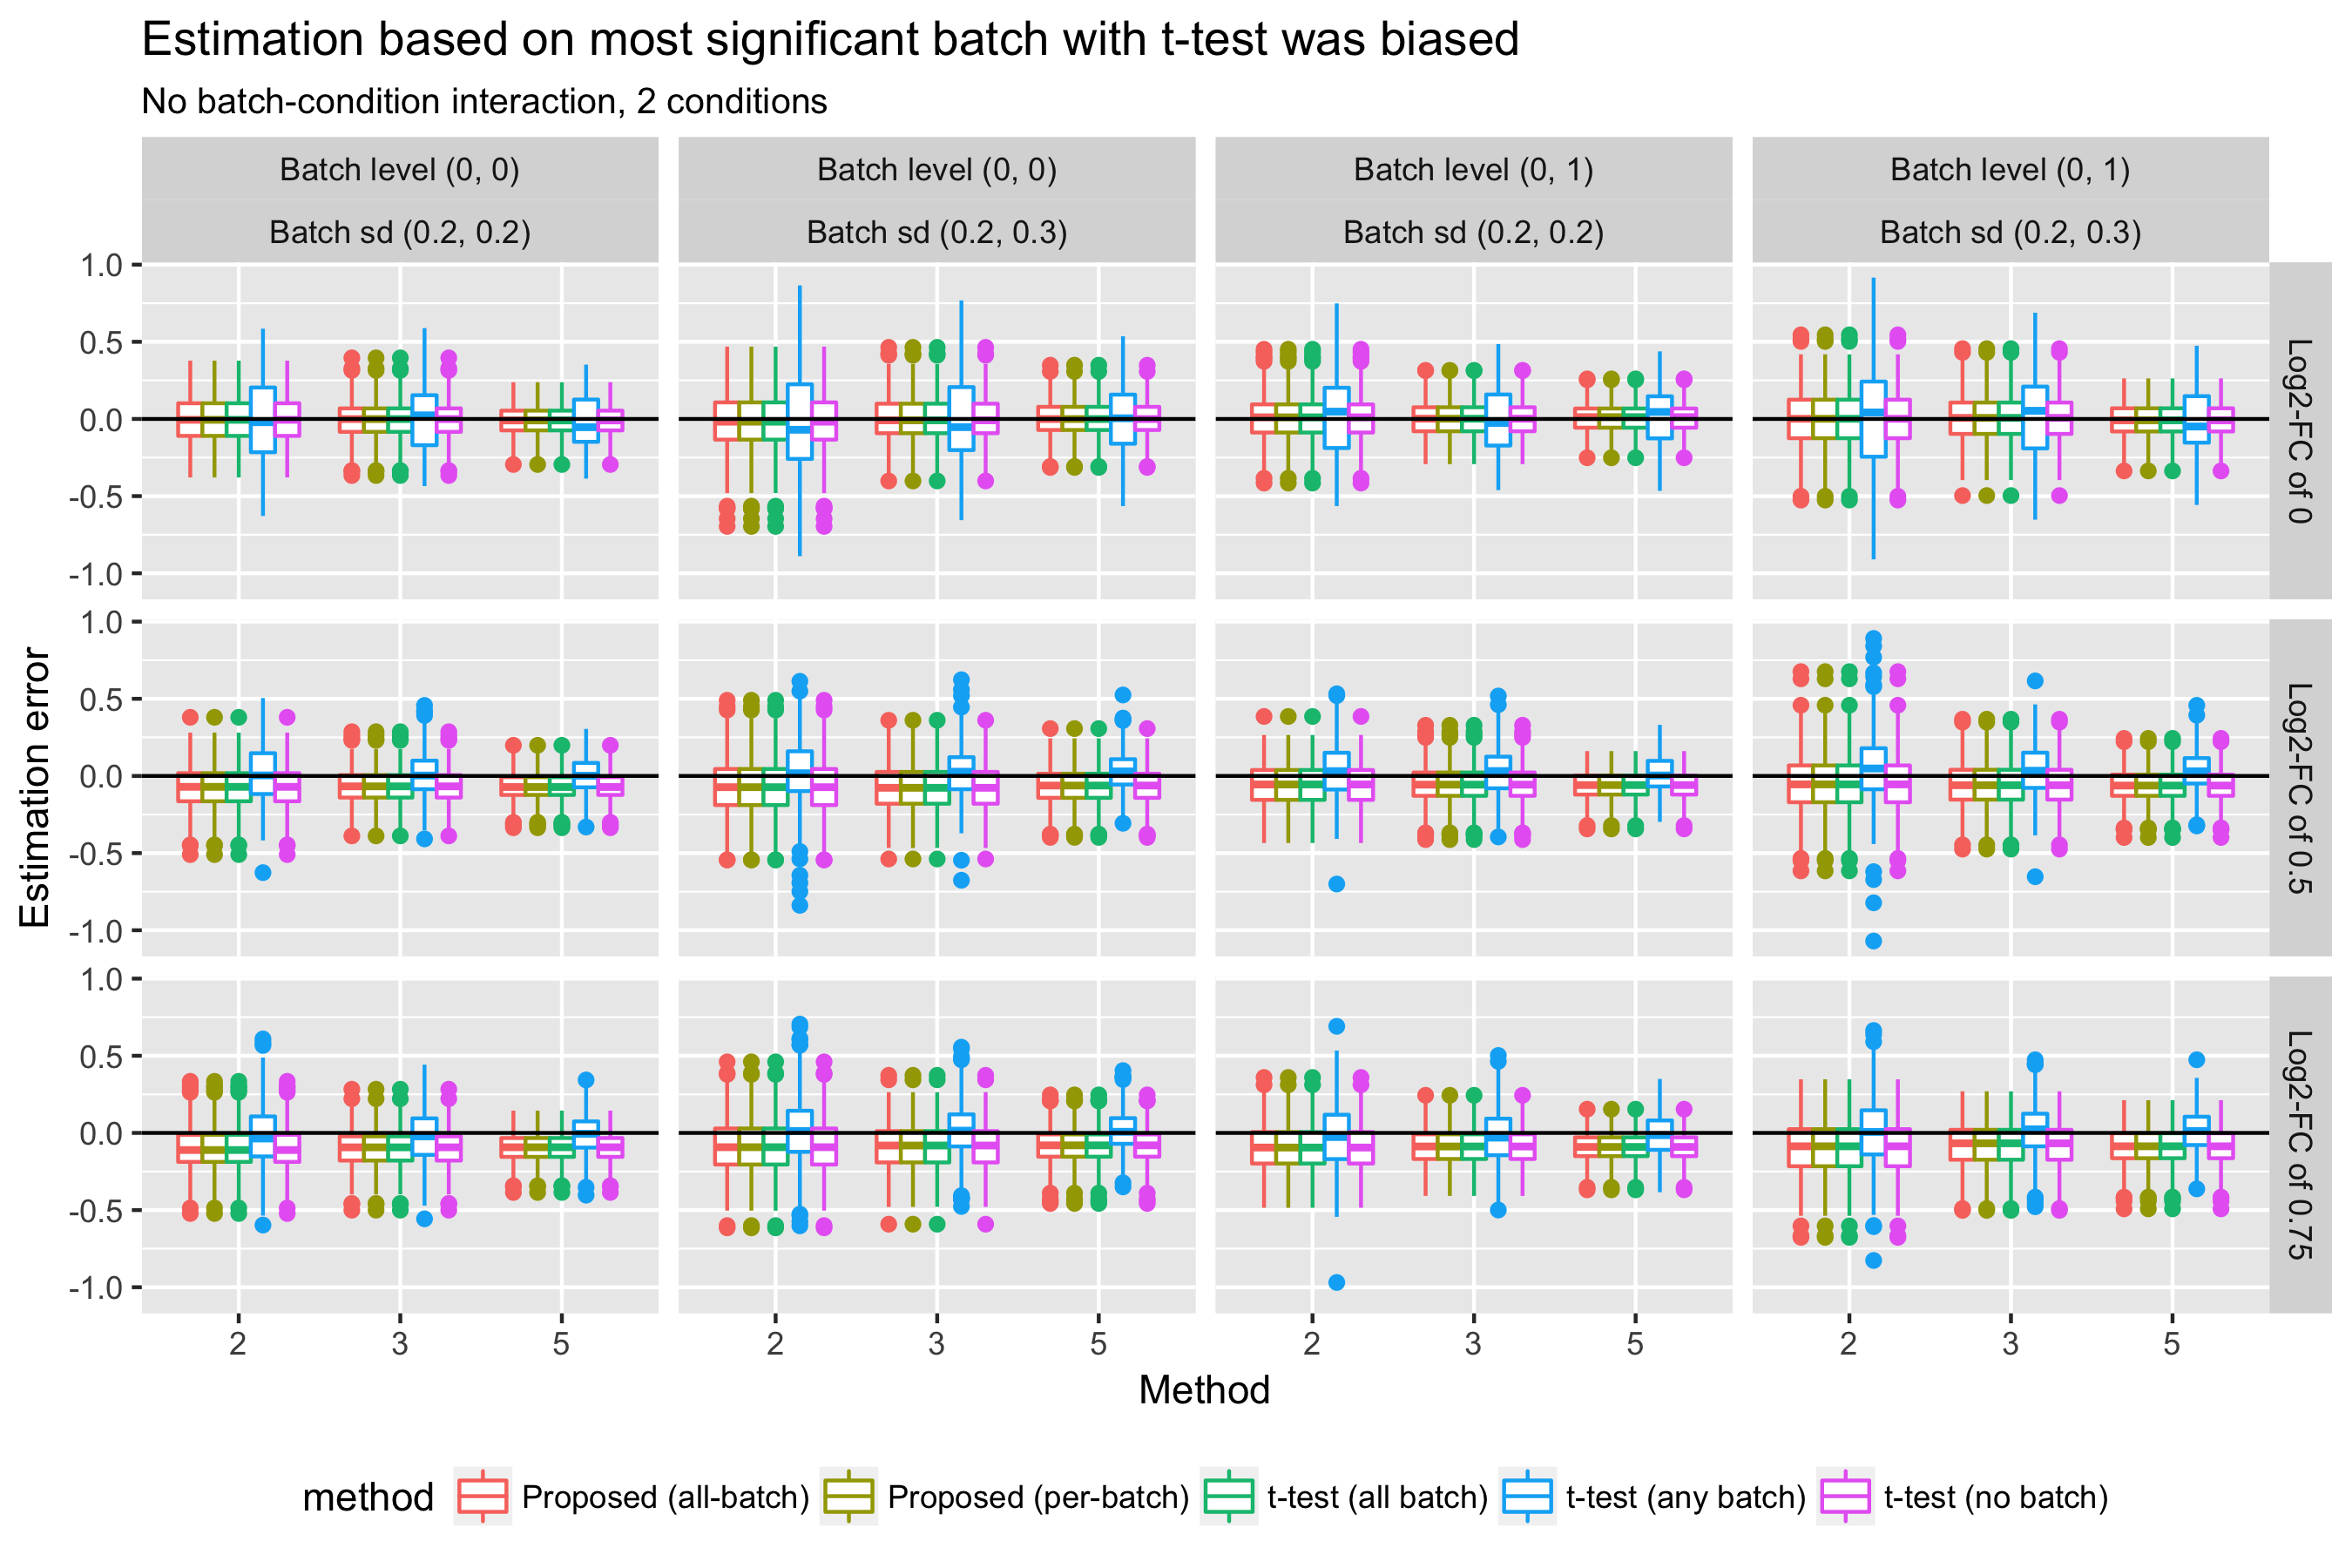
\includegraphics[width=.825\textwidth]{sim/synnull_est_2}
\caption{Estiamtion based on the most statistically significant batch with $t$-test was highly variable and frequently biased. The observation is consistent in all the simulated scenarios. \label{fig:synnull_est}}
\end{figure}

\begin{figure}[h!]
\centering
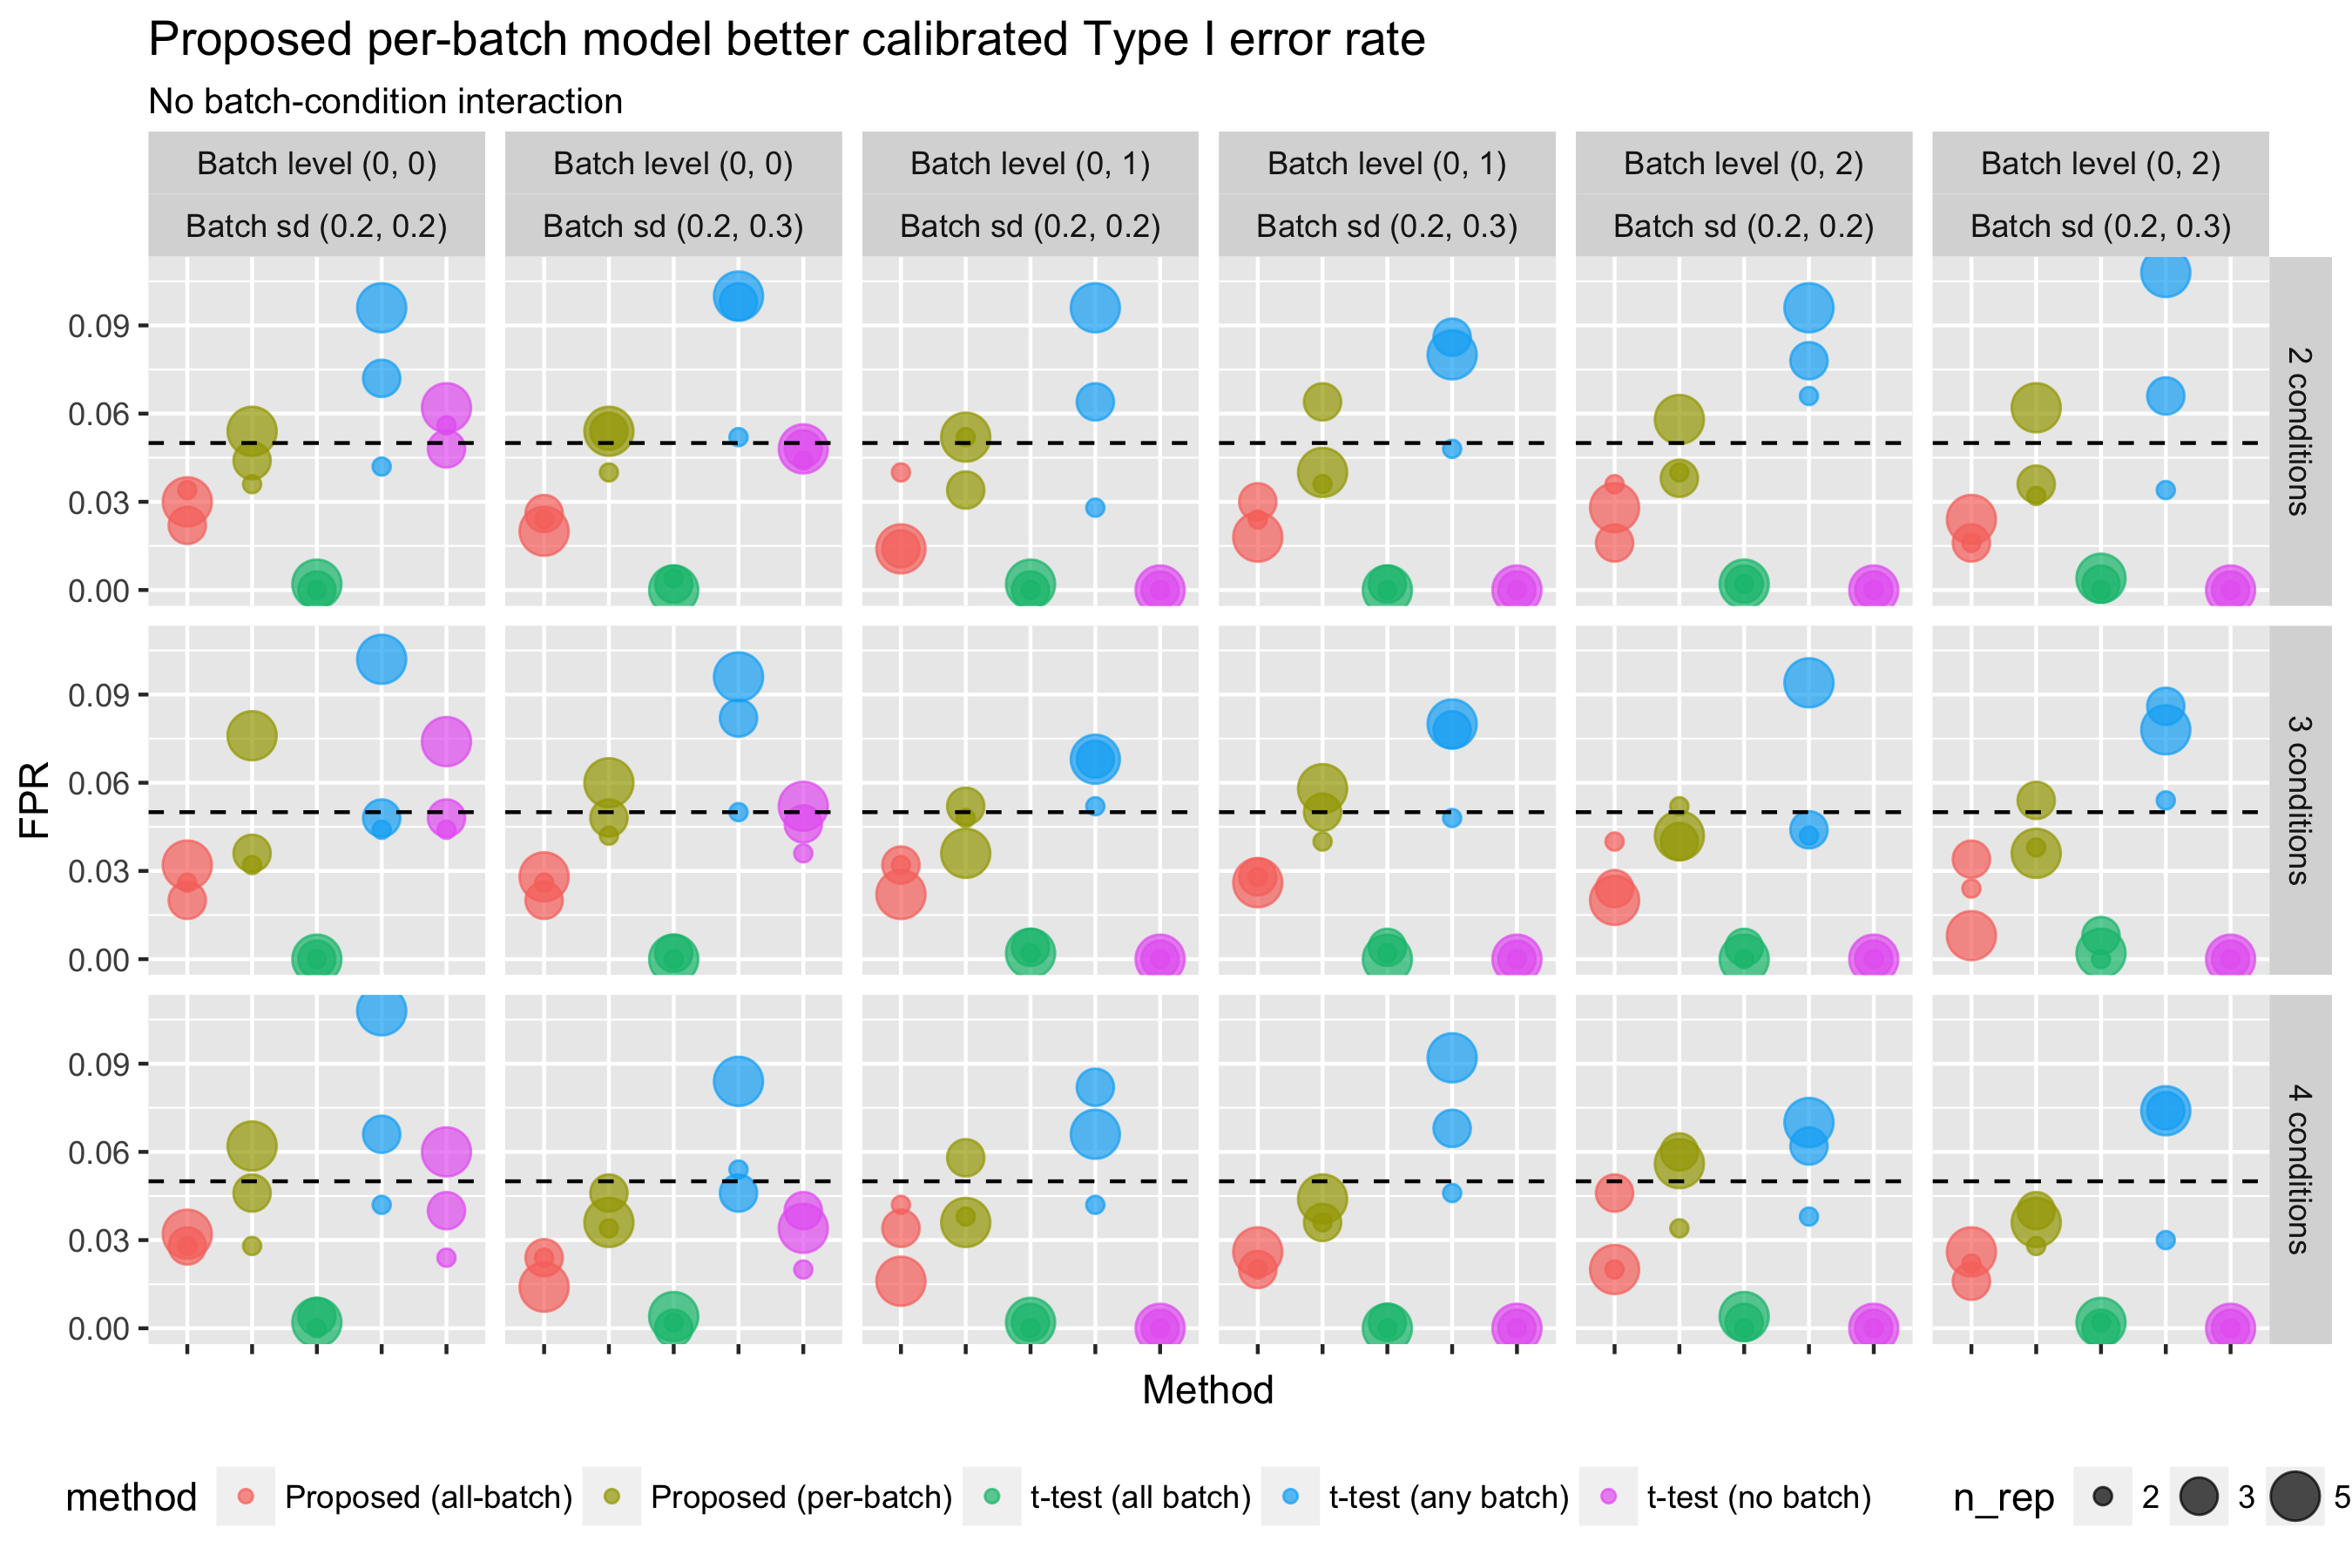
\includegraphics[width=.825\textwidth]{sim/synnull_fpr}
\caption{The proposed per-batch model better calibrated Type I error rate. Similar results were observed in the cases with positive and negative interactions. \label{fig:synnull_fpr}}
\end{figure}


\clearpage
\begin{figure}[h!]
\centering
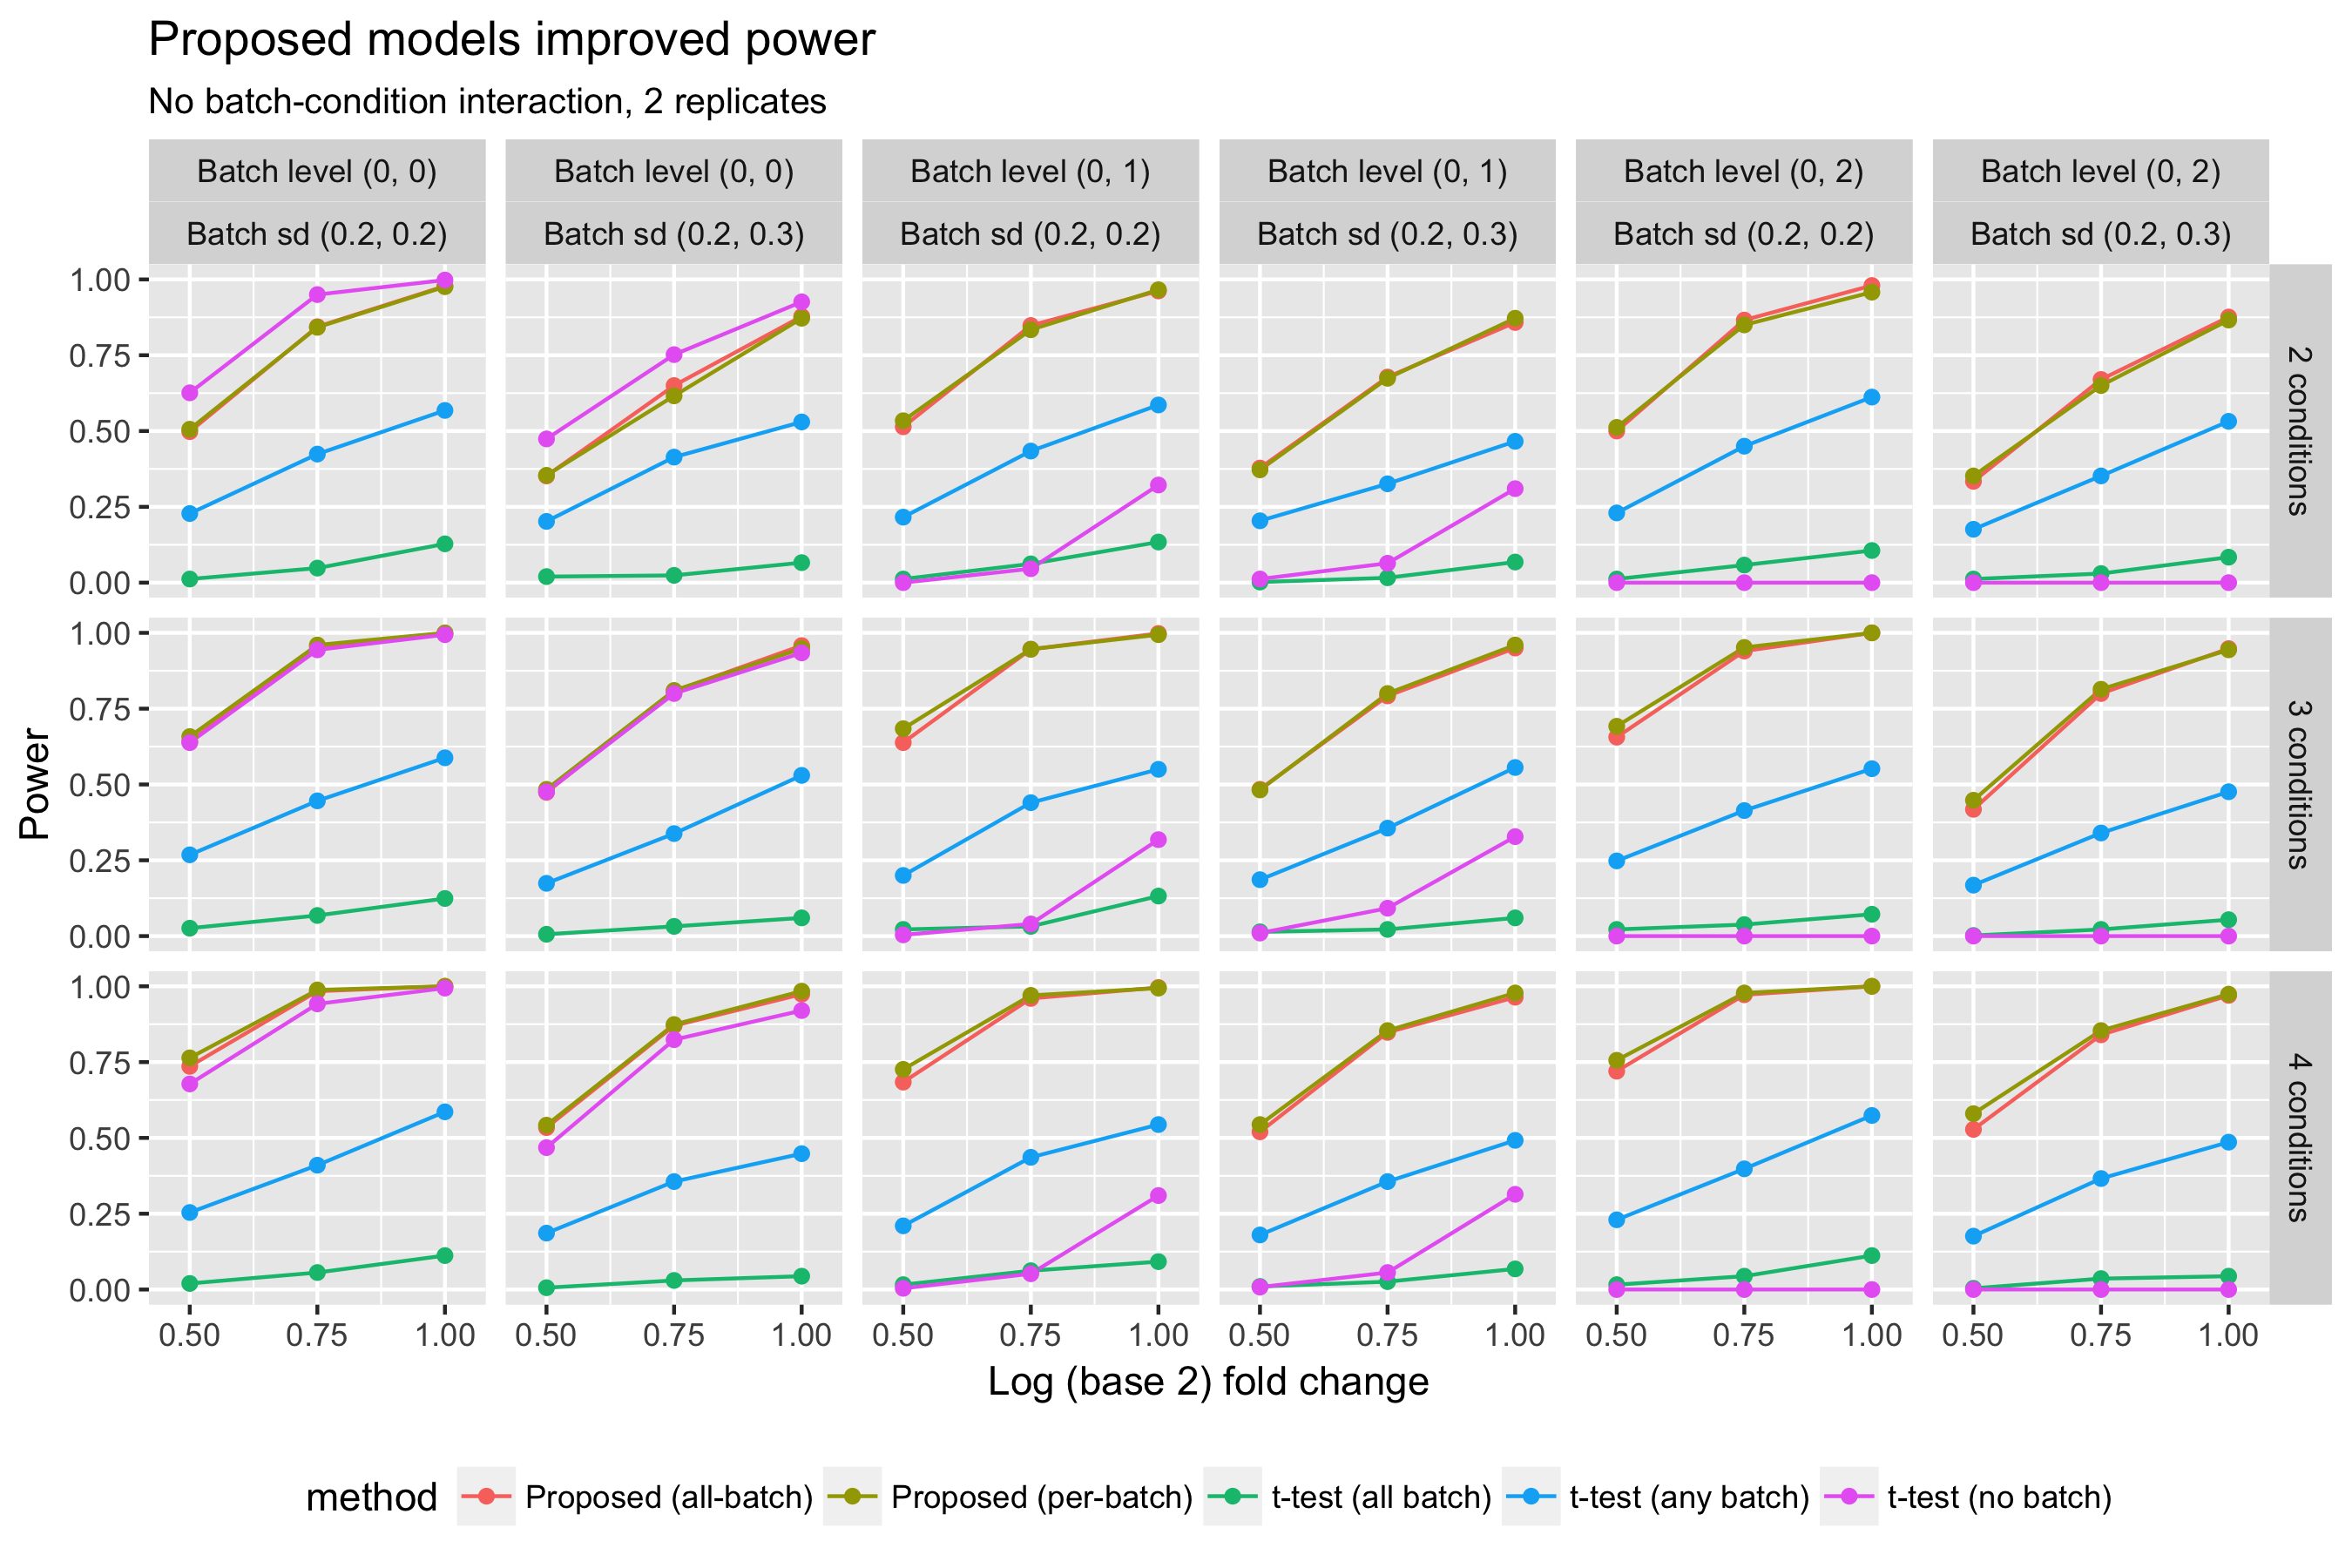
\includegraphics[width=.85\textwidth]{sim/synnull_pwr_2}\\
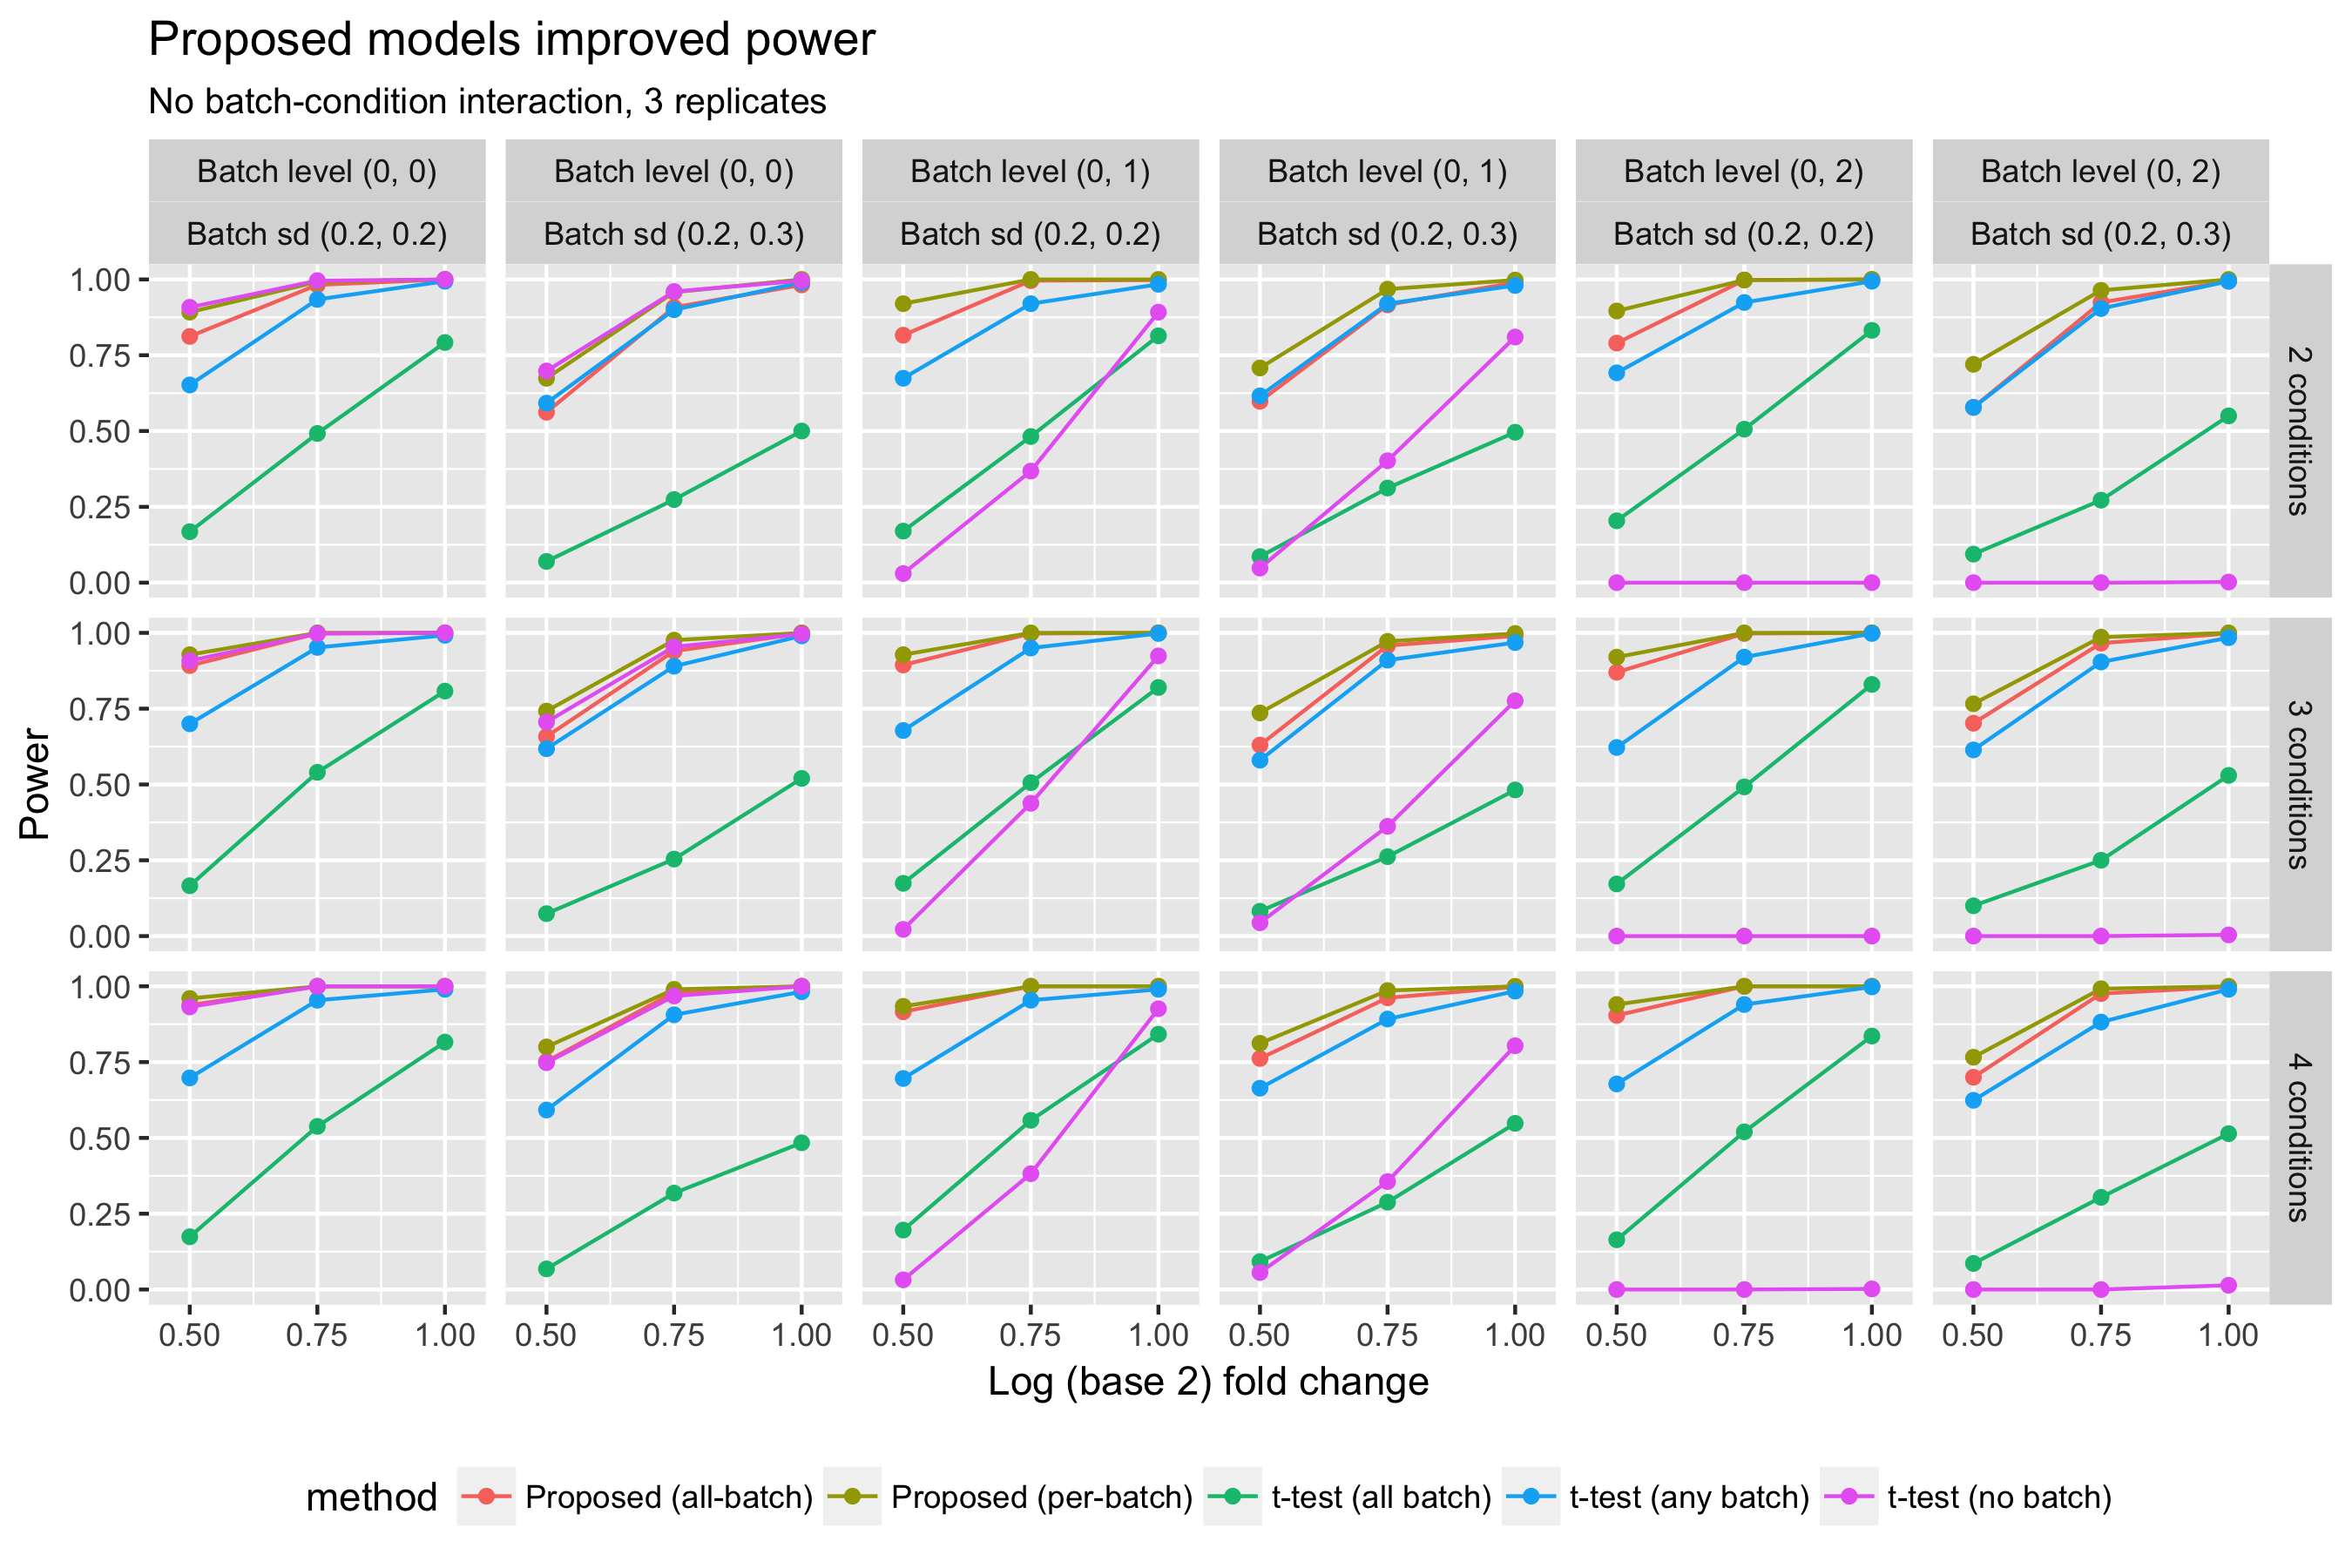
\includegraphics[width=.85\textwidth]{sim/synnull_pwr_3}
\caption{The proposed model improved power with small sample sizes in almost all the scenarios, under various forms of batch effects including difference in intensity level (higher on the right) and difference in variability. Using $t$-test while ignoring batch effect gave similar performance in special cases with no difference in intensity level between batches, but its performance dramatically decreased in general cases. The proposed methods gave consistently improved performance compared with other methods by properly characterizing batch effects and leveraging all available information. \label{fig:synnull_pwr}}
\end{figure}


\clearpage
\begin{figure}[h!]
\centering
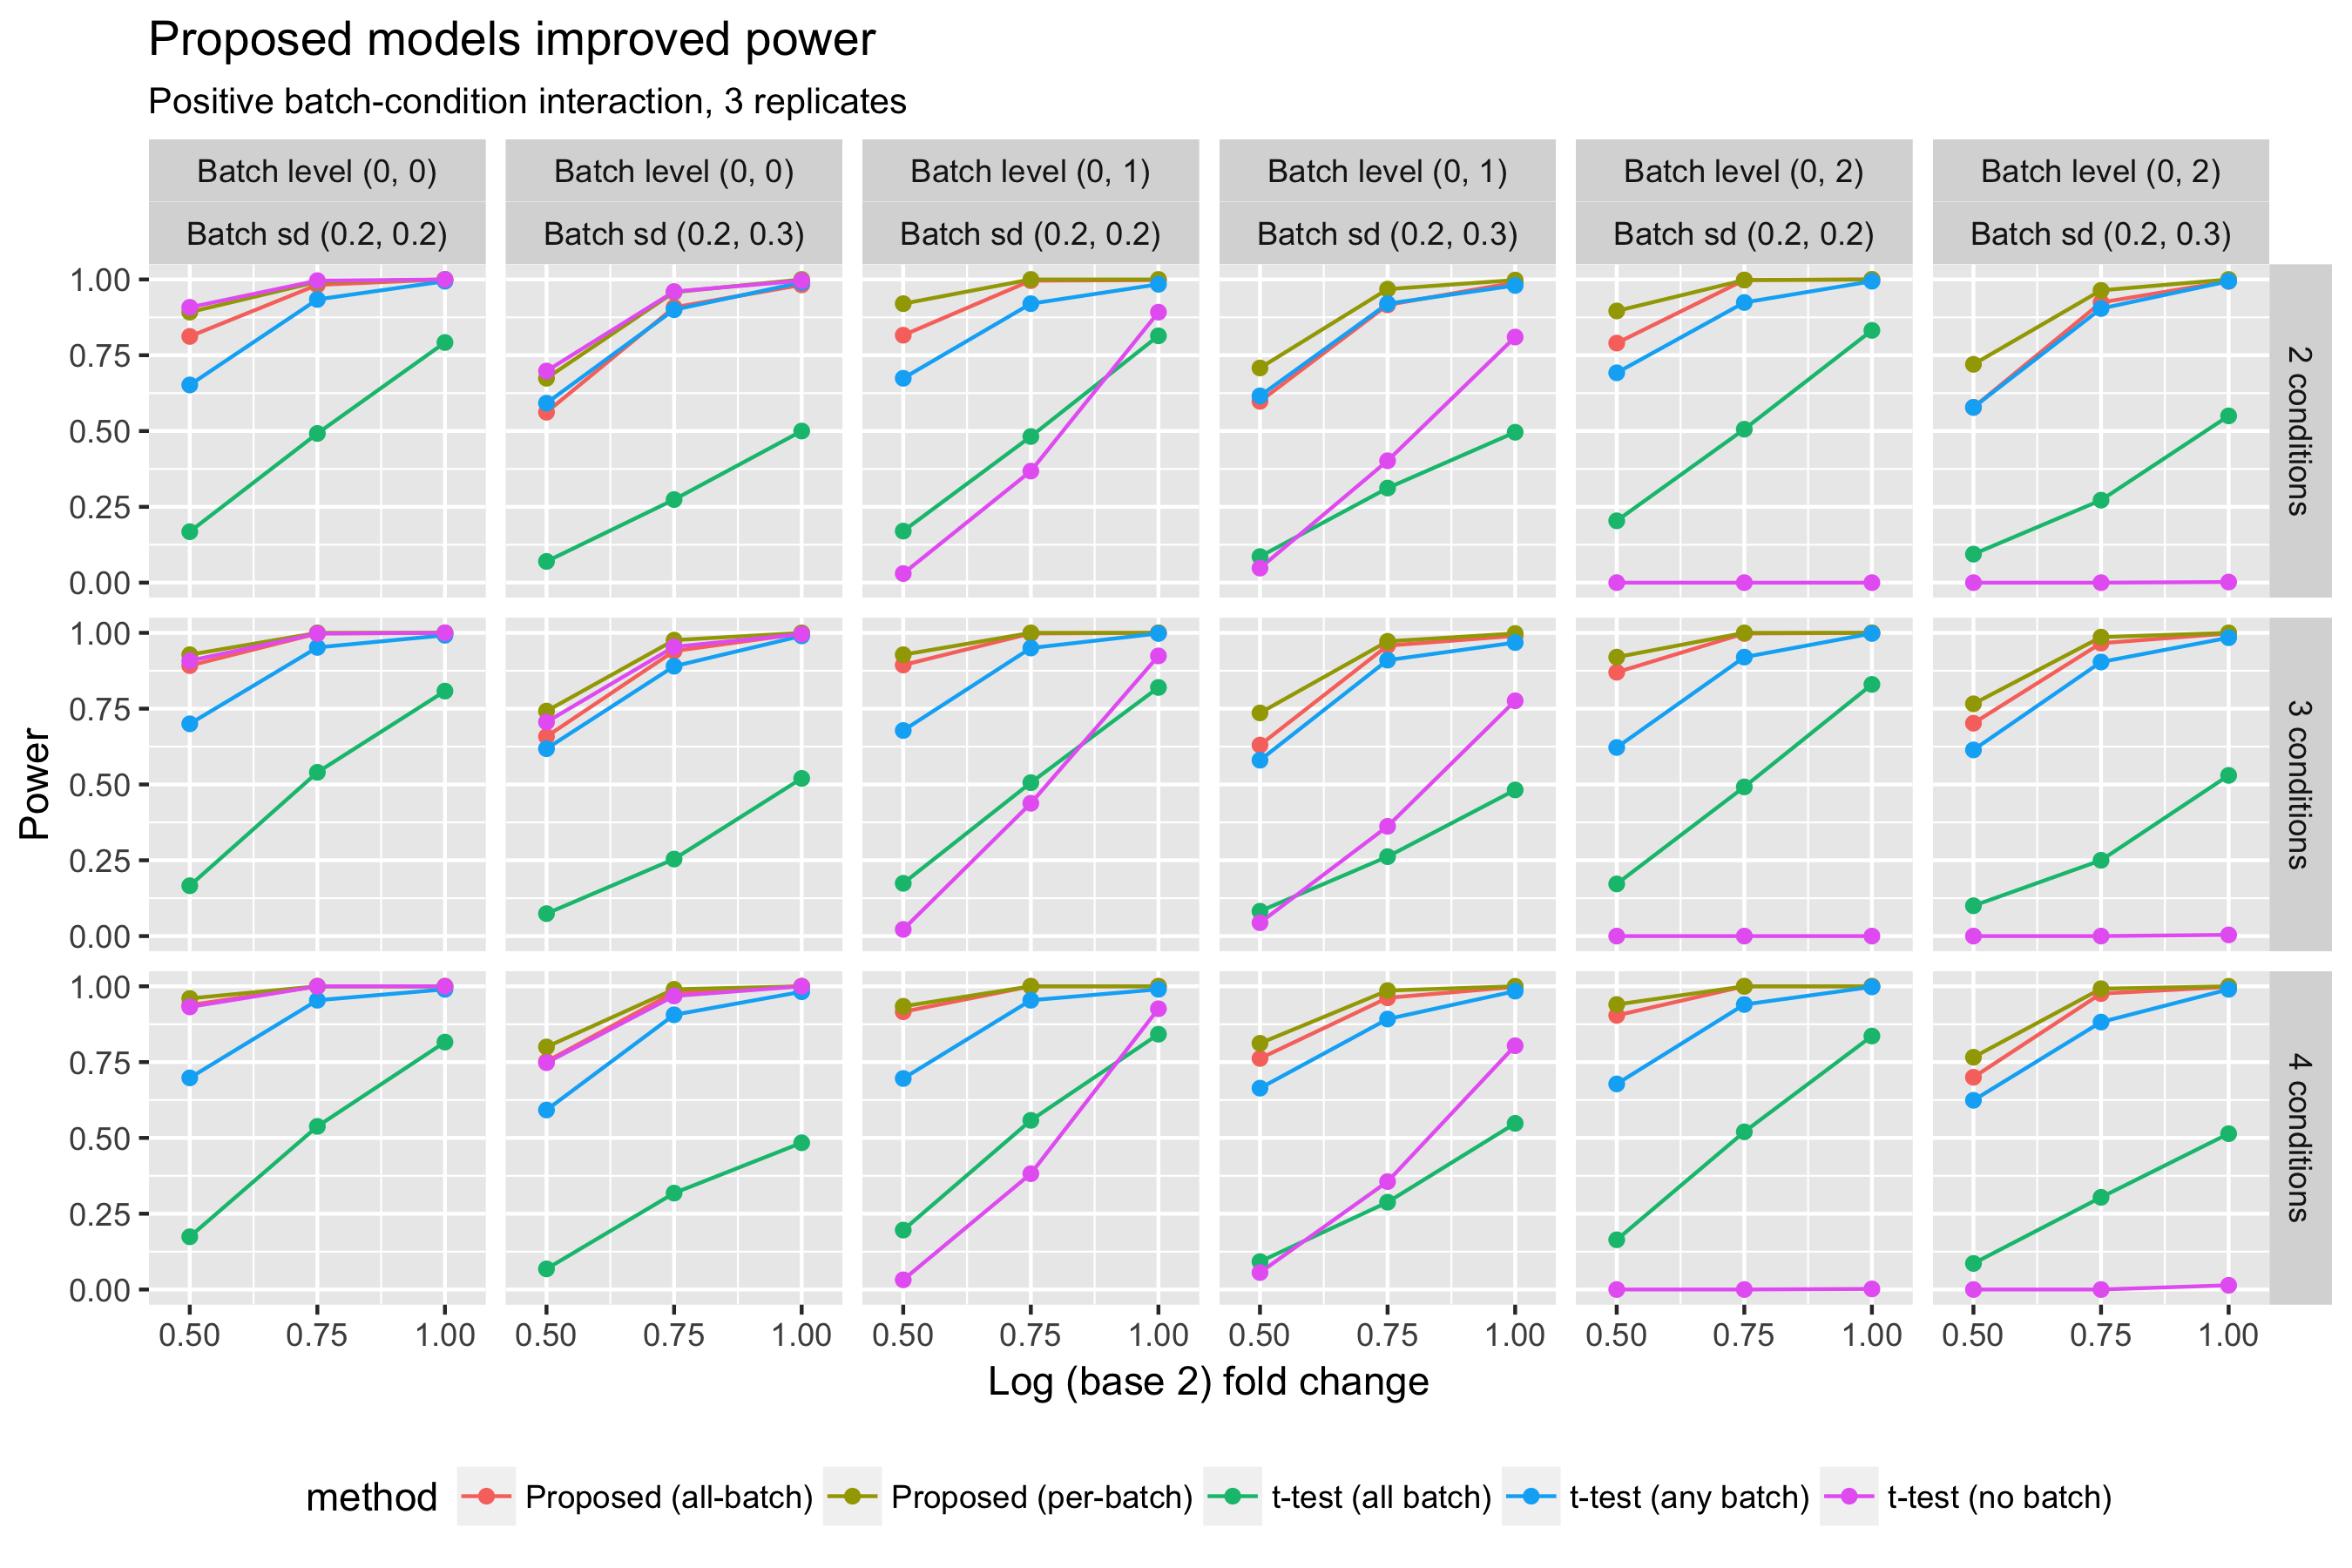
\includegraphics[width=.85\textwidth]{sim/synpos_pwr_3}\\
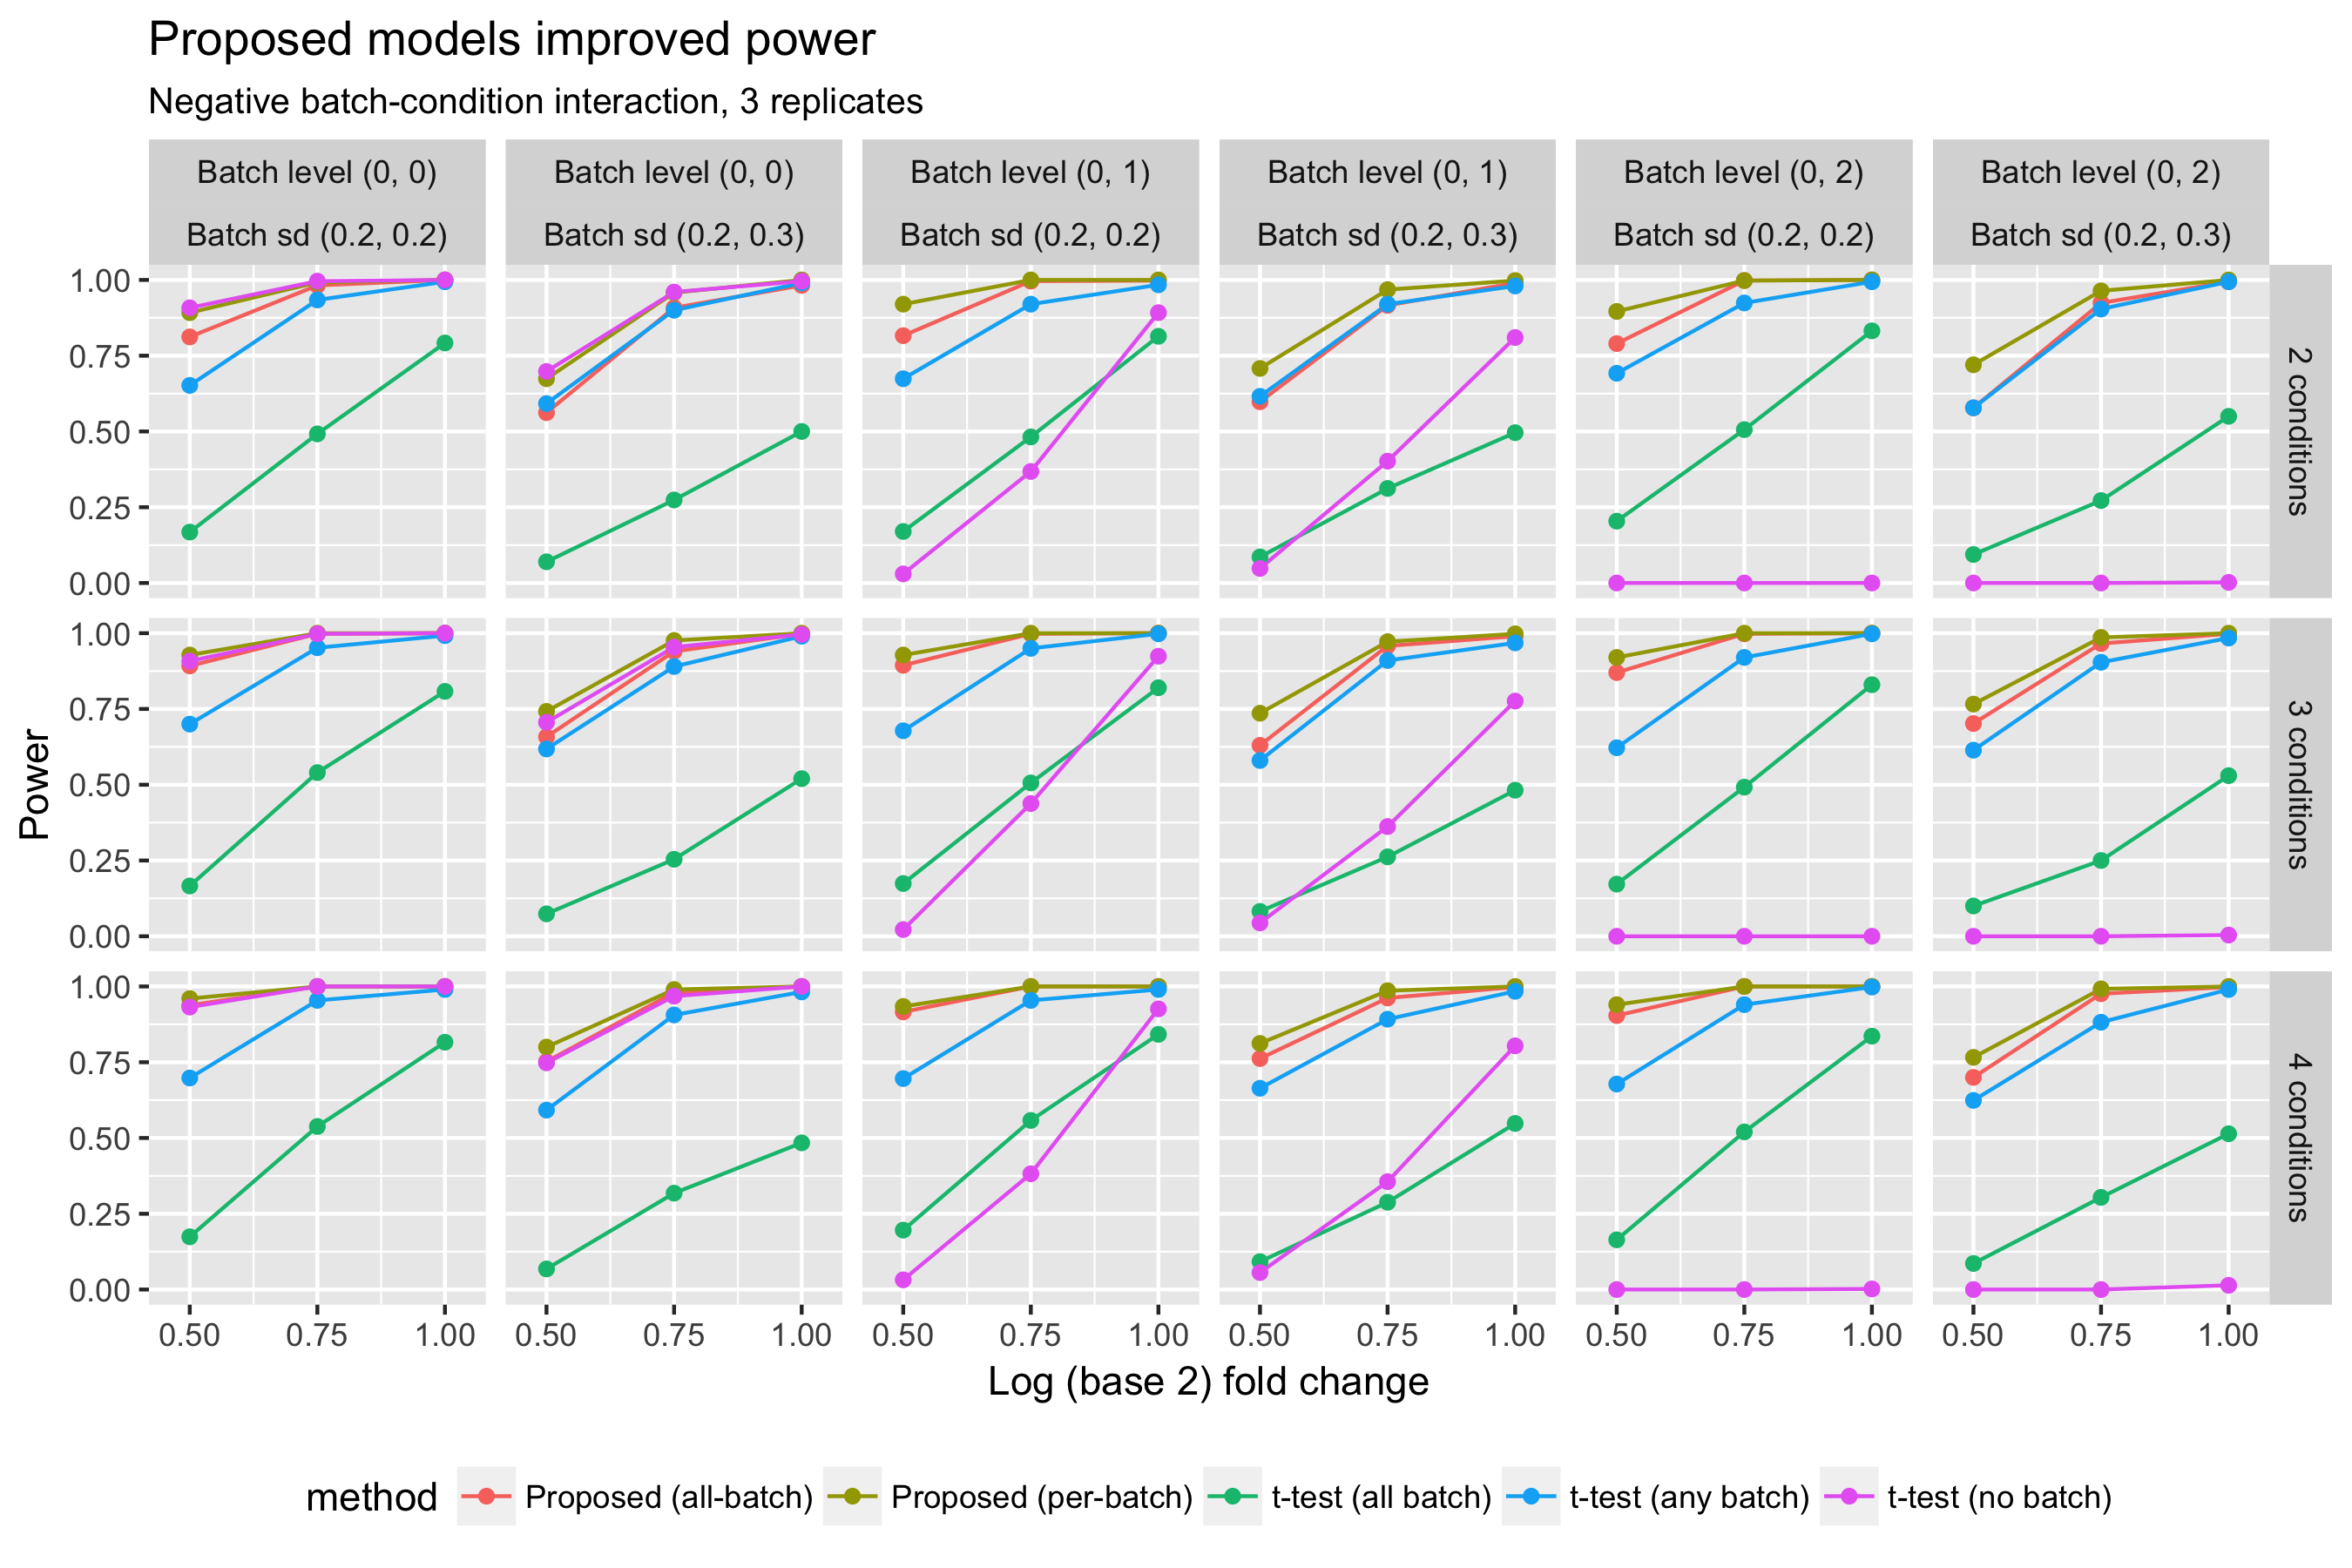
\includegraphics[width=.85\textwidth]{sim/synneg_pwr_3}
\caption{With 3 replicates and under the scenarios with either positive or negative interaction, the proposed models consistently improved power over other methods. Similar results were observed with 2 replicates. As in those cases with no interaction, the approaches using two-sample $t$-test did not benefit from data in additional conditions. Also, ignoring batch effects as applying $t$-test (no batch) lost power dramatically. \label{fig:syn_pwr_3}}
\end{figure}


\begin{figure}[h!]
\centering
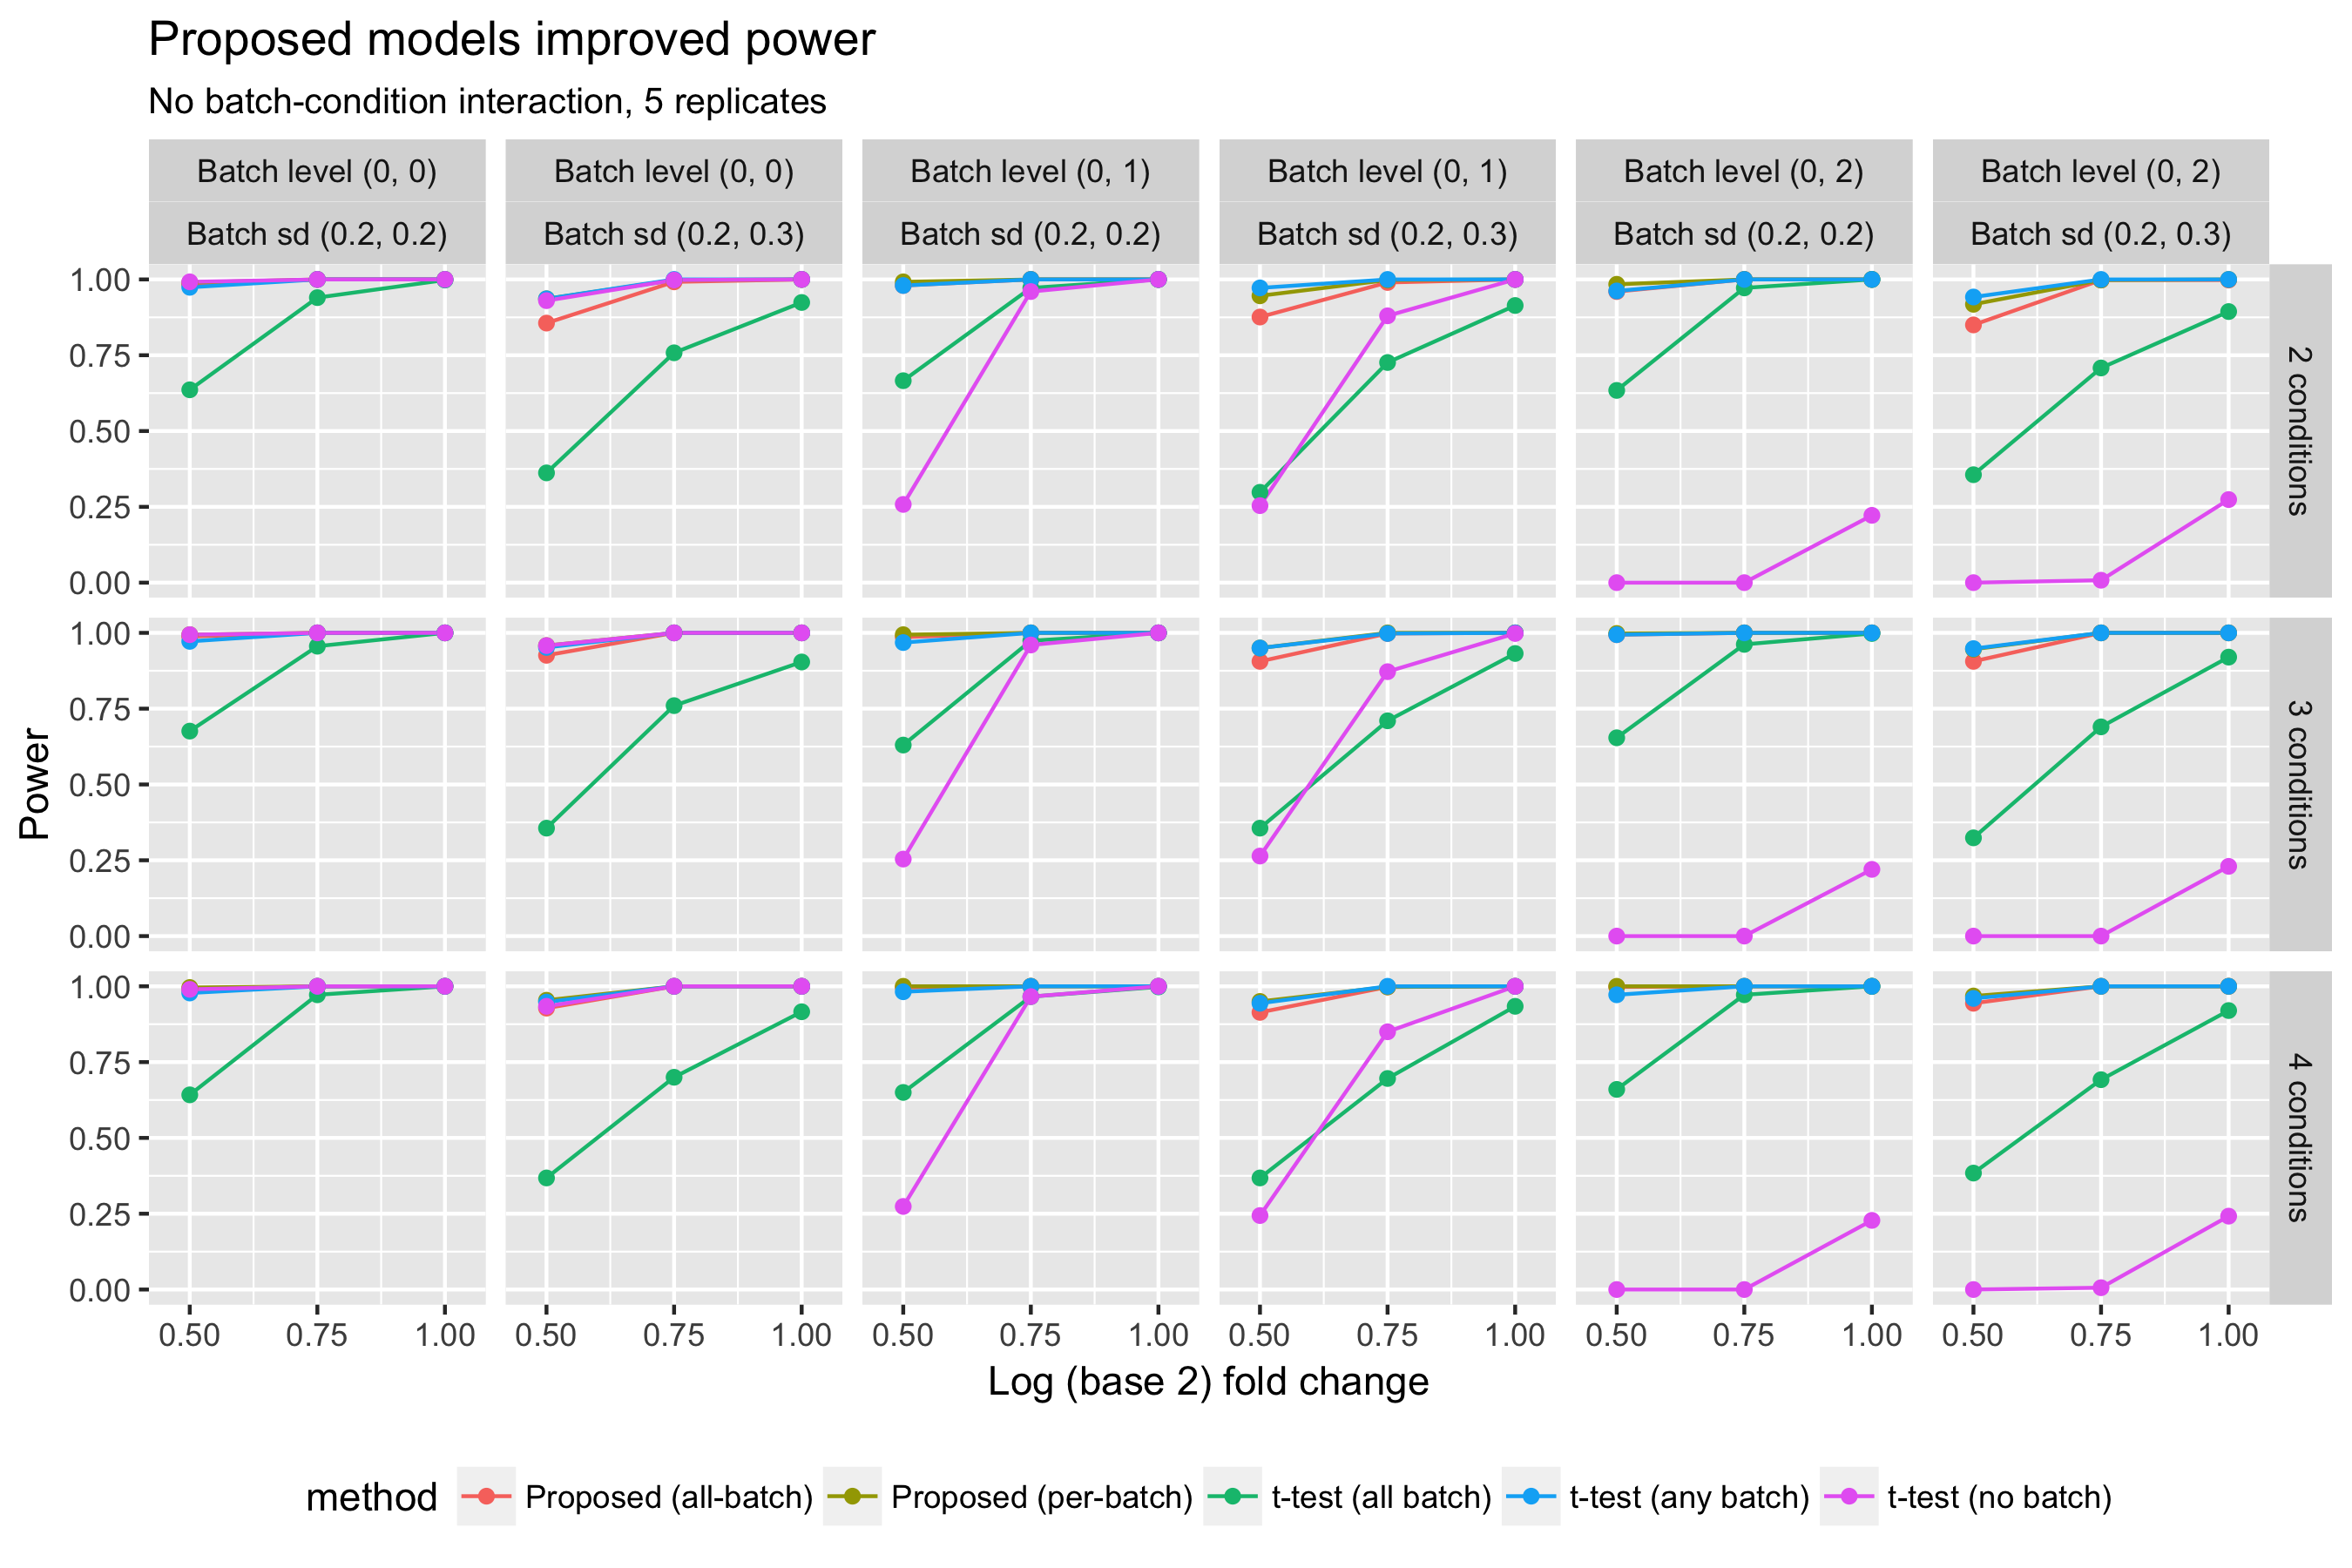
\includegraphics[width=.85\textwidth]{sim/synnull_pwr_5}
\caption{Ignoring batch effects lost power. The negative impact was only partially reduced by increasing the sample size to 5. Similar patterns were observed in other simulated scenarios. \label{fig:synnull_pwr_5}}
\end{figure}


\clearpage
%%%%%%%%%%%%%%%%%%%%%%%%%%%%%%%%%%%%%%%%%%%%%%%%%%%%%%%%%%%%%%%%
\subsection{Protein-level adjustment}

%%%%%%%%%%%%%%%%%%%%%%%%%%%%%%%%%%%%%%%%%%%%%%%%%%%%%%%%%%%%%%%%
\subsubsection{One site per protein}

Differential levels of modified peptides may be due to changes in modification or change in protein abundance. Adjustment with respect to unmodified peptides can correct for the confounding factor, with a cost of increased uncertainty. We evaluated such adjustment by computer simulation. Below are the parameters used in the simulation: 
\begin{itemize}
\item Mean of log-intensity: $25$
\item Standard deviations of log-intensity of modified peptides: 
\begin{itemize}
\item Identical variances across batches: $0.2$ in both Batch 1 and Batch 2
\item Different variances across batches: $0.2$ and $0.3$ in Batch 1 and Batch 2, respectively
\end{itemize}
\item Standard deviations of log-intensity of unmodified peptides: $0.2$ in both batches
\item Difference in modification level between conditions: $0$, $0.5$
\item Difference in protein level between conditions: $0$, $0.5$
\item Number of replicates: $2$, $3$, $5$
\item Number of conditions: $2$, $3$, $4$
\item Number of realizations: $500$
\end{itemize}

\begin{figure}[h!]
\centering
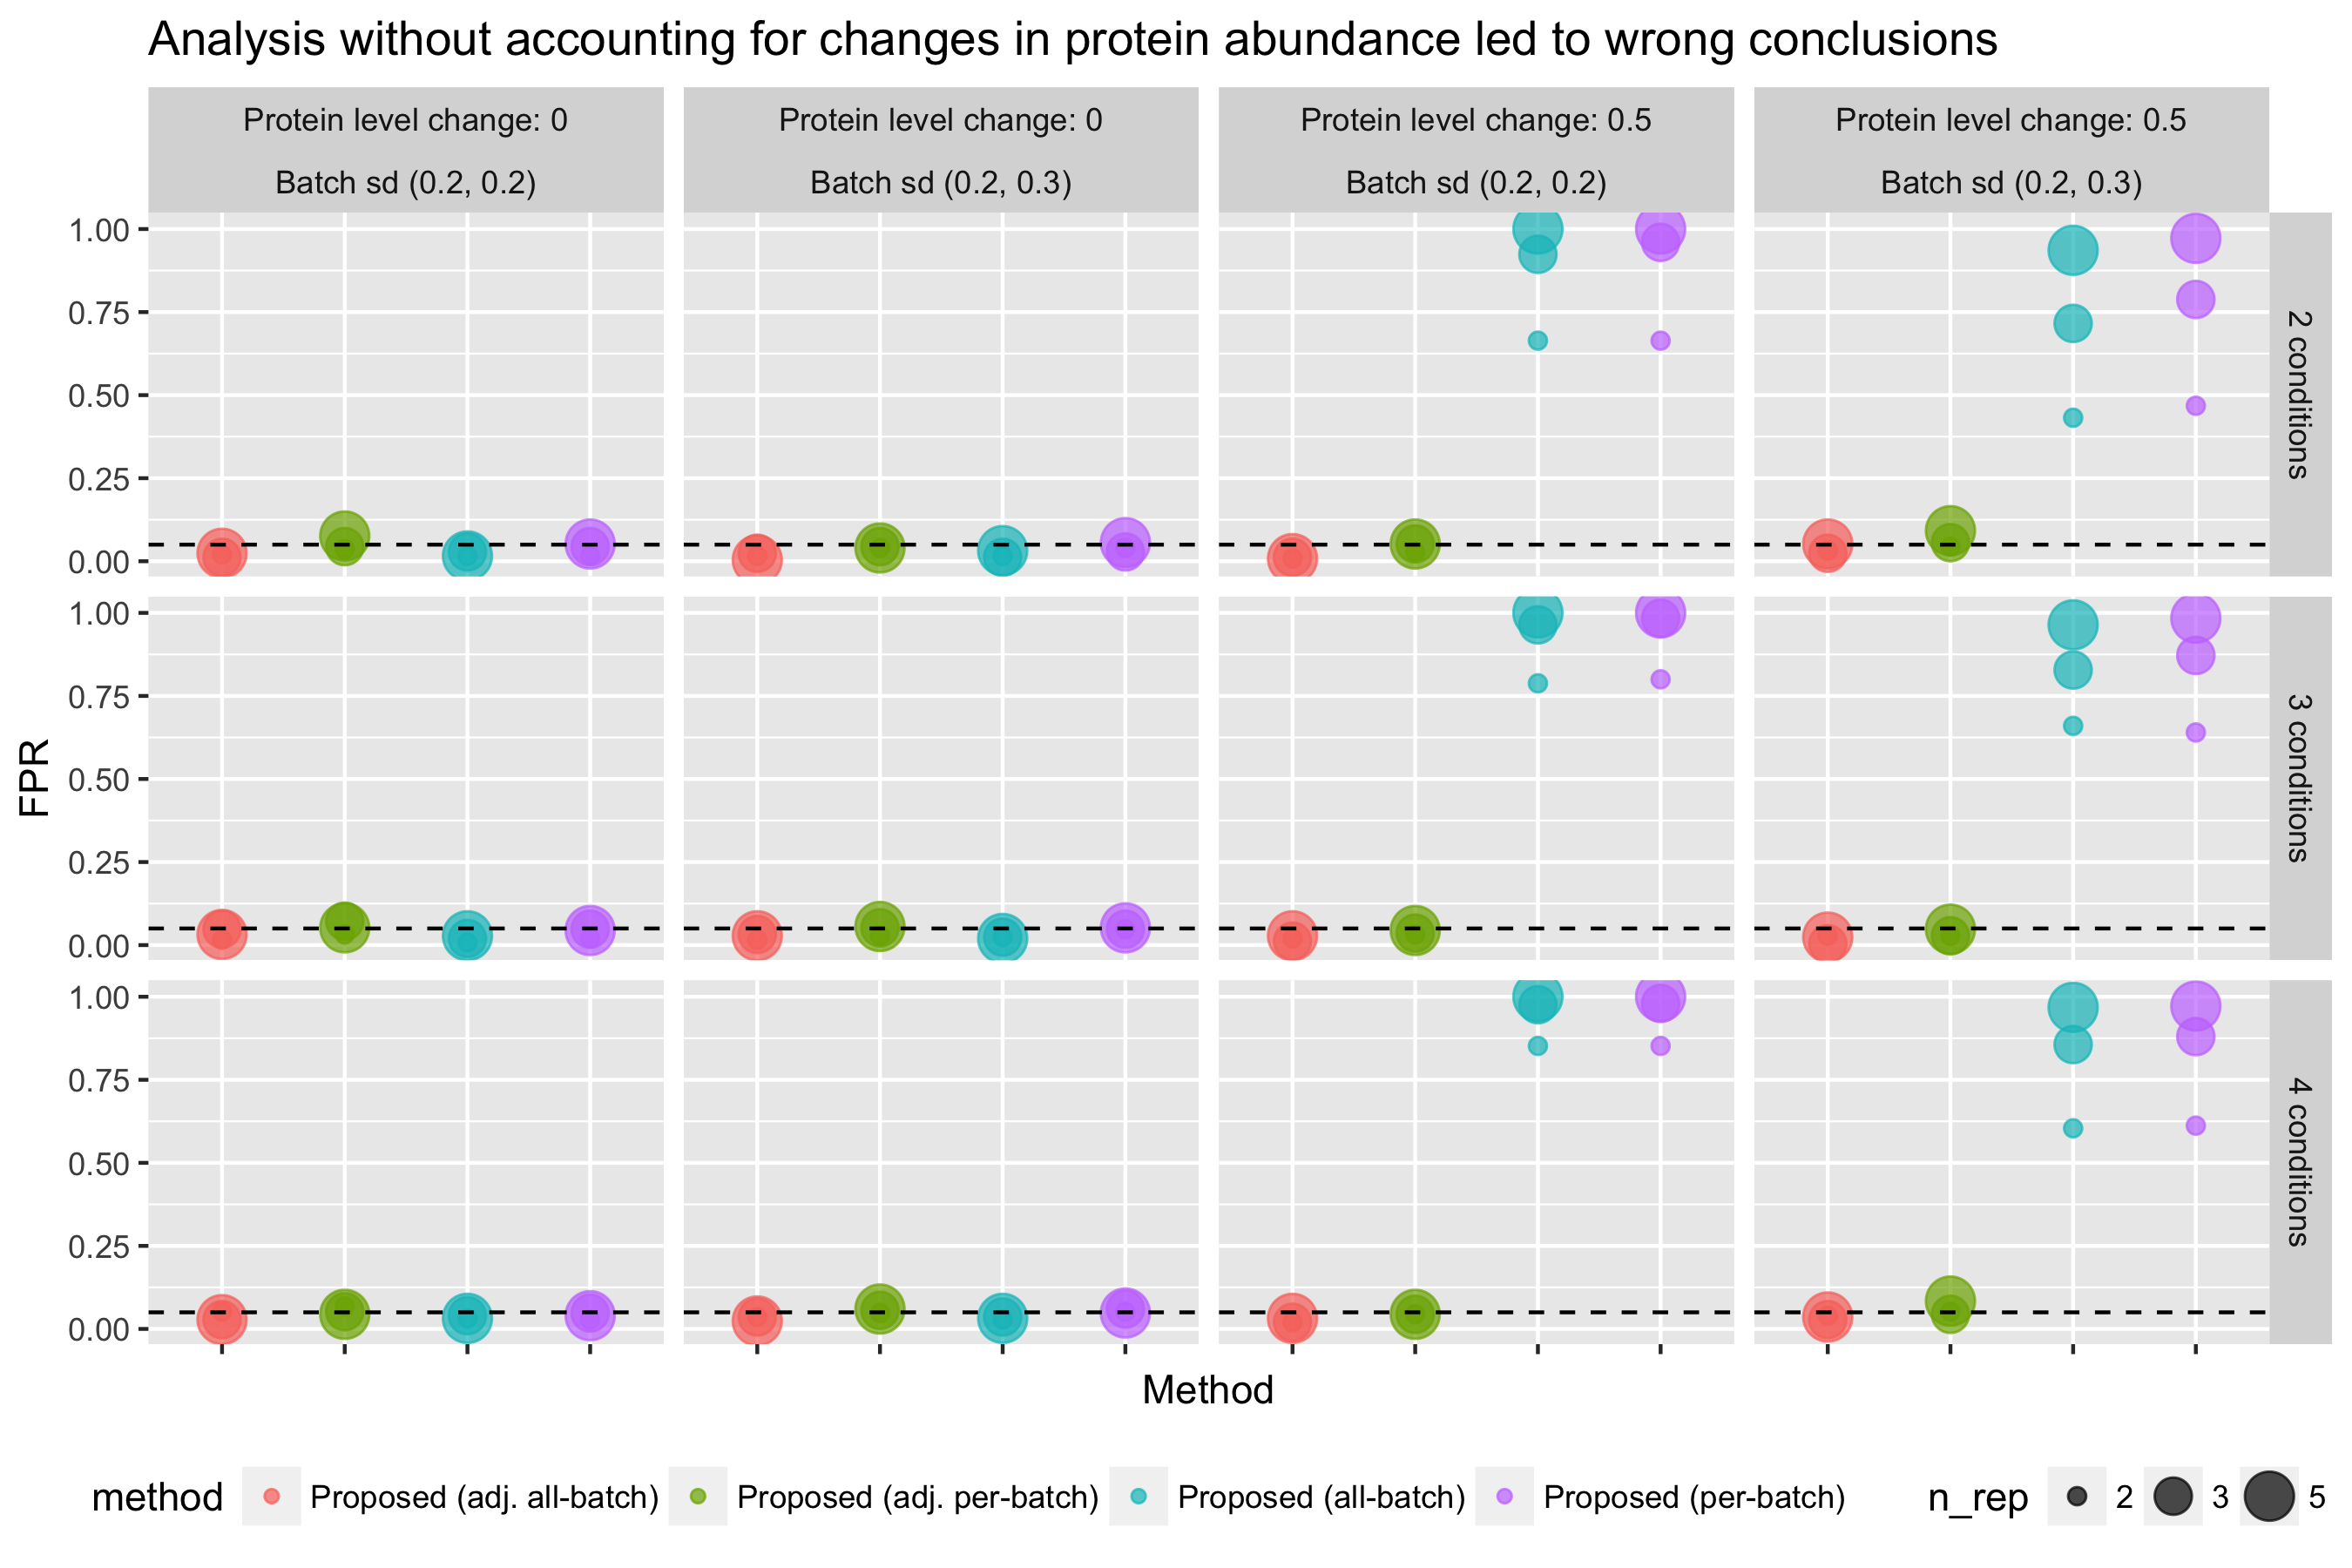
\includegraphics[width=.85\textwidth]{sim/prot_fpr}
\caption{
All the proposed methods well calibrated the Type I error rate when there was no change in protein abundance (leftmost two columns). When the modification changes were entirely due to the changes in protein abundance across conditions, analysis without accounting for the protein-level changes resulted in off-target, high false positive rates. \label{fig:prot_fpr}}
\end{figure}


\begin{figure}[h!]
\centering
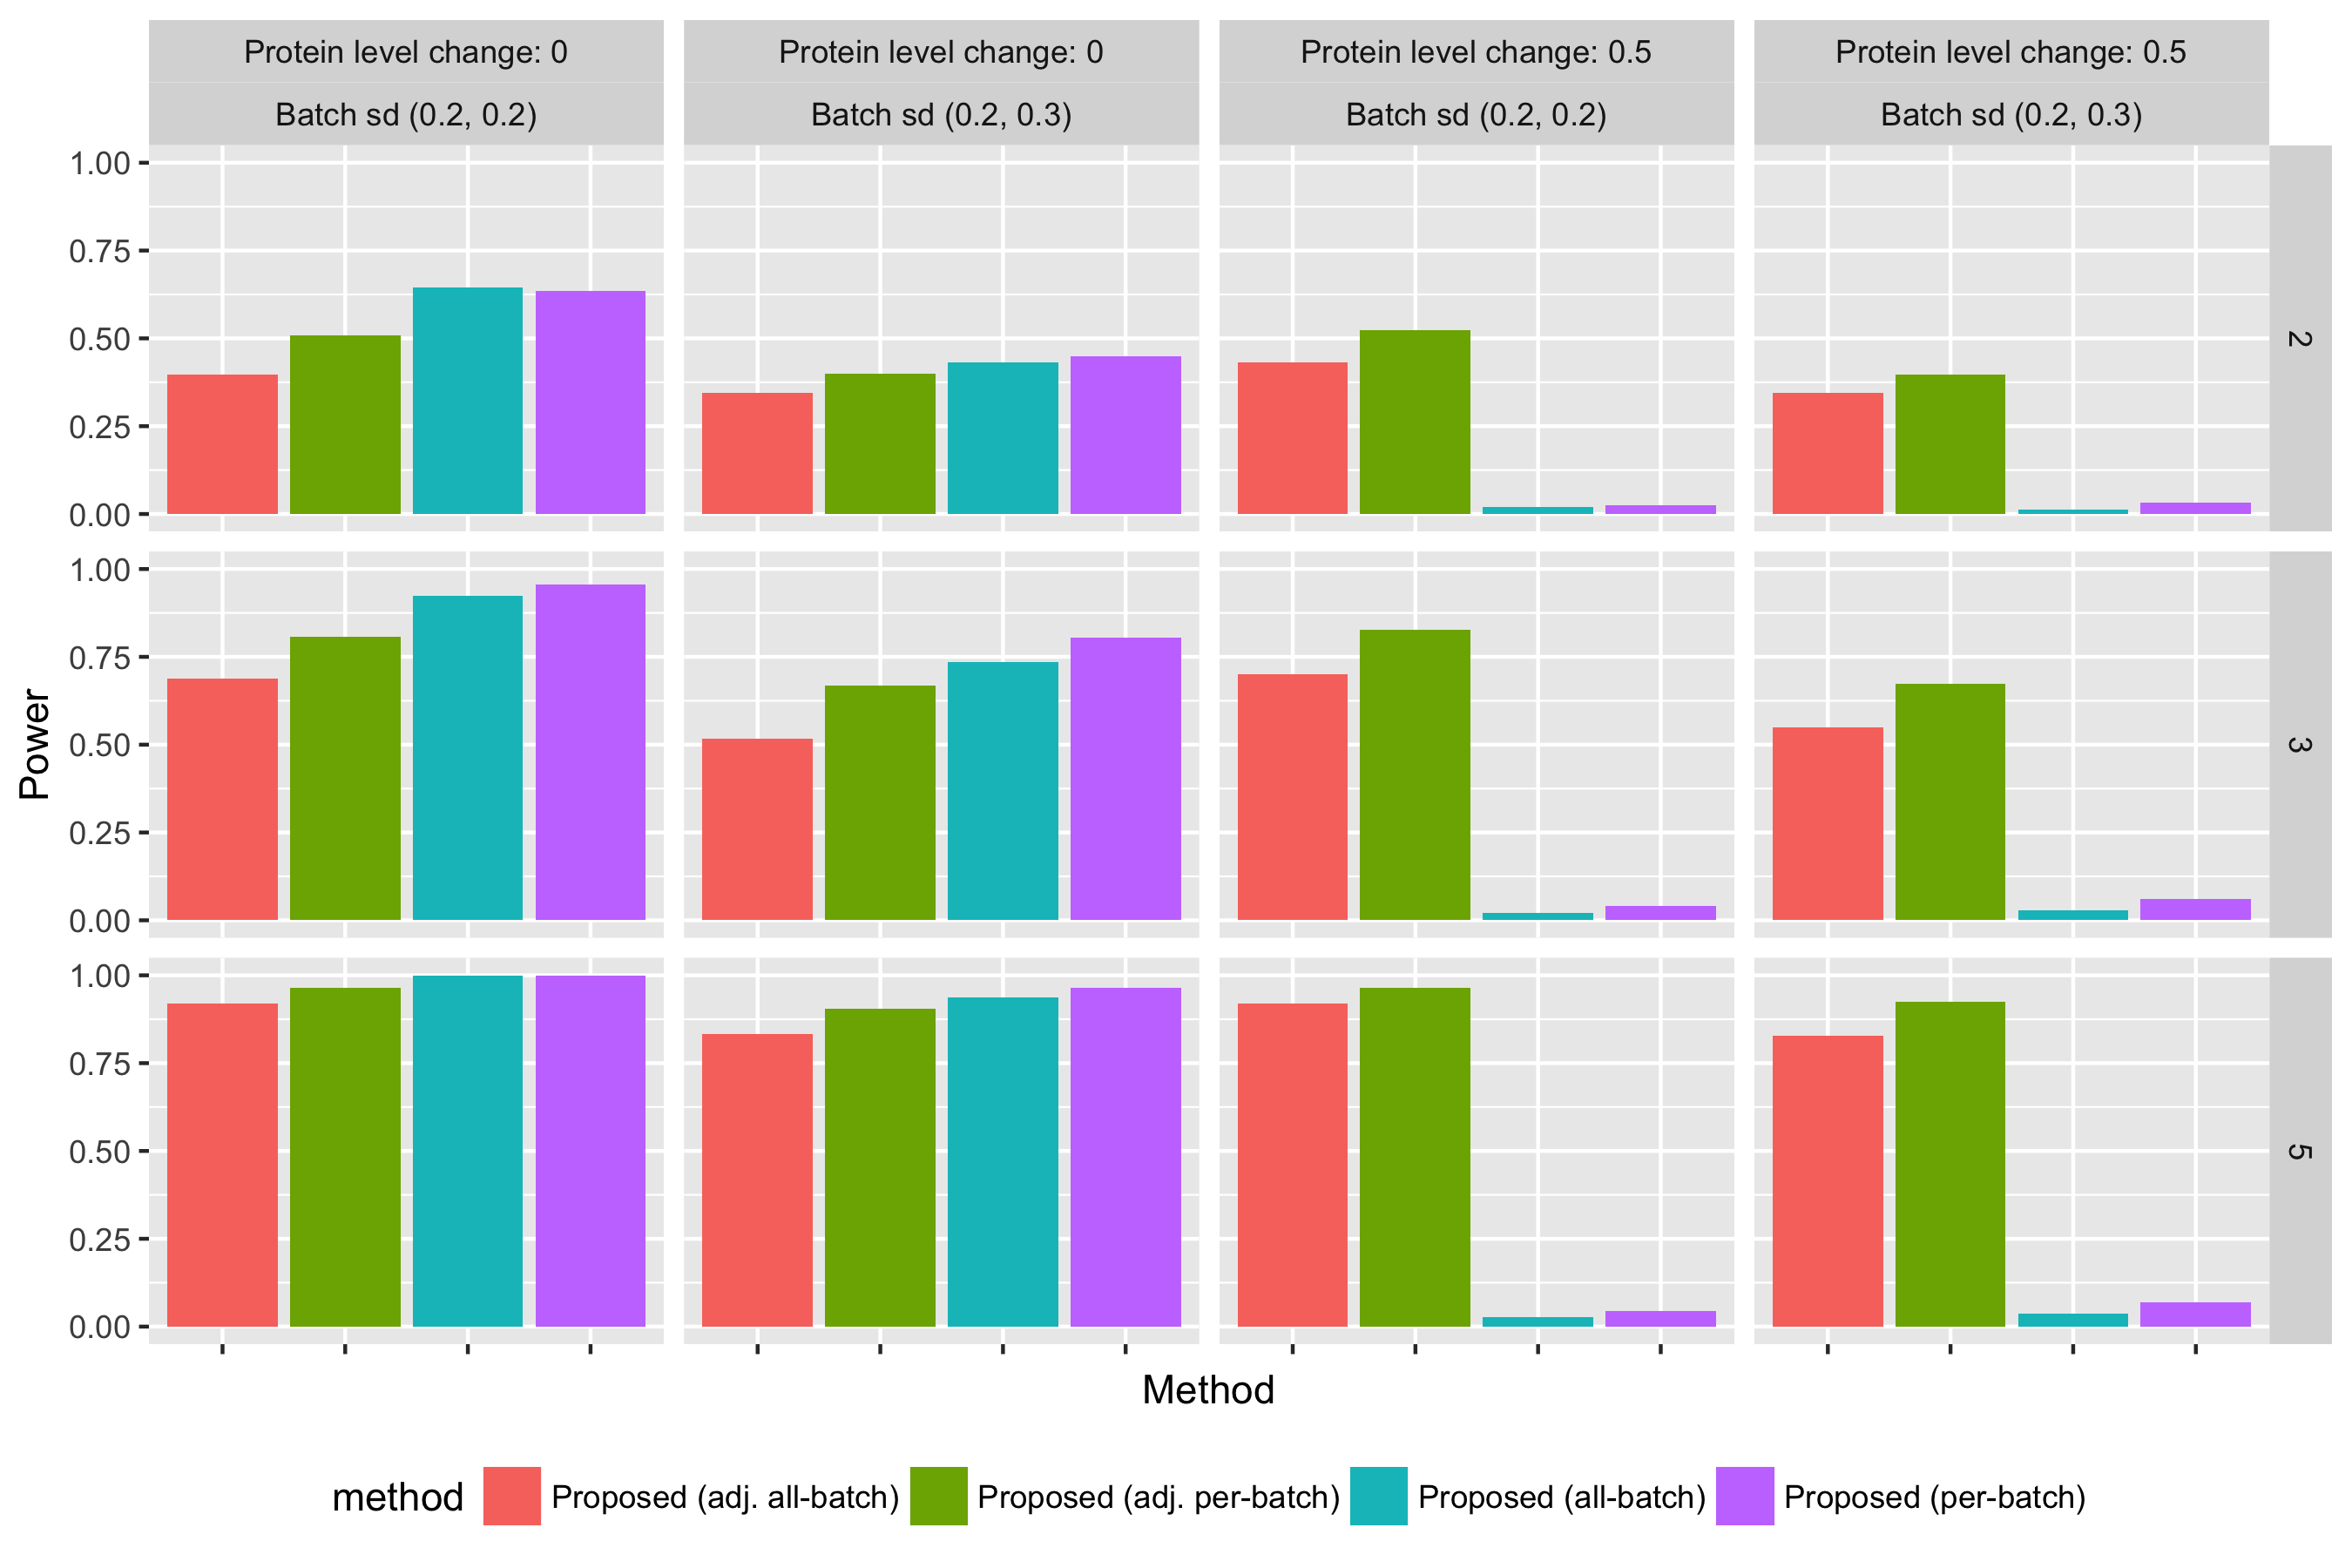
\includegraphics[width=.85\textwidth]{sim/prot_pwr}
\caption{Adjustment with respect to unmodified peptides increase uncertainty in the estimation and testing. When there was no change in protein abundance (leftmost two columns), the approaches with no adjustment resulted in slightly higher power. However, their performances decreased significantly when such confounding indeed existed (rightmost two columns). \label{fig:prot_pwr}}
\end{figure}


%%%%%%%%%%%%%%%%%%%%%%%%%%%%%%%%%%%%%%%%%%%%%%%%%%%%%%%%%%%%%%%%
\subsubsection{Multiple sites per protein}

Expression levels of modification sites are adjusted based on the abundance of their originating protein. Since the same reference is used for all the sites, it introduces correlation between estimates and test statistics for those sites. This may cause issues in controlling false discovery rate (FDR). We investigated the property by simulating data of two conditions and 1000 proteins with different numbers of modification sites. A fraction (50\% or 80\%) of the 1000 proteins had no changes between conditions while systematic changes were simulated for the rest of the proteins. Multiple testing correction was performed using the Benjamini and Hochberg's method. Performances of the considered approaches were assessed by their power and FDR. The power was calculated as the fraction of proteins with adjusted $p$-values $<0.05$ among those proteins with true differences between conditions, while the FDR was calculated as the fraction of proteins with adjusted $p$-values $<0.05$ among the proteins with true differences. 

 
\begin{figure}[h!]
\centering
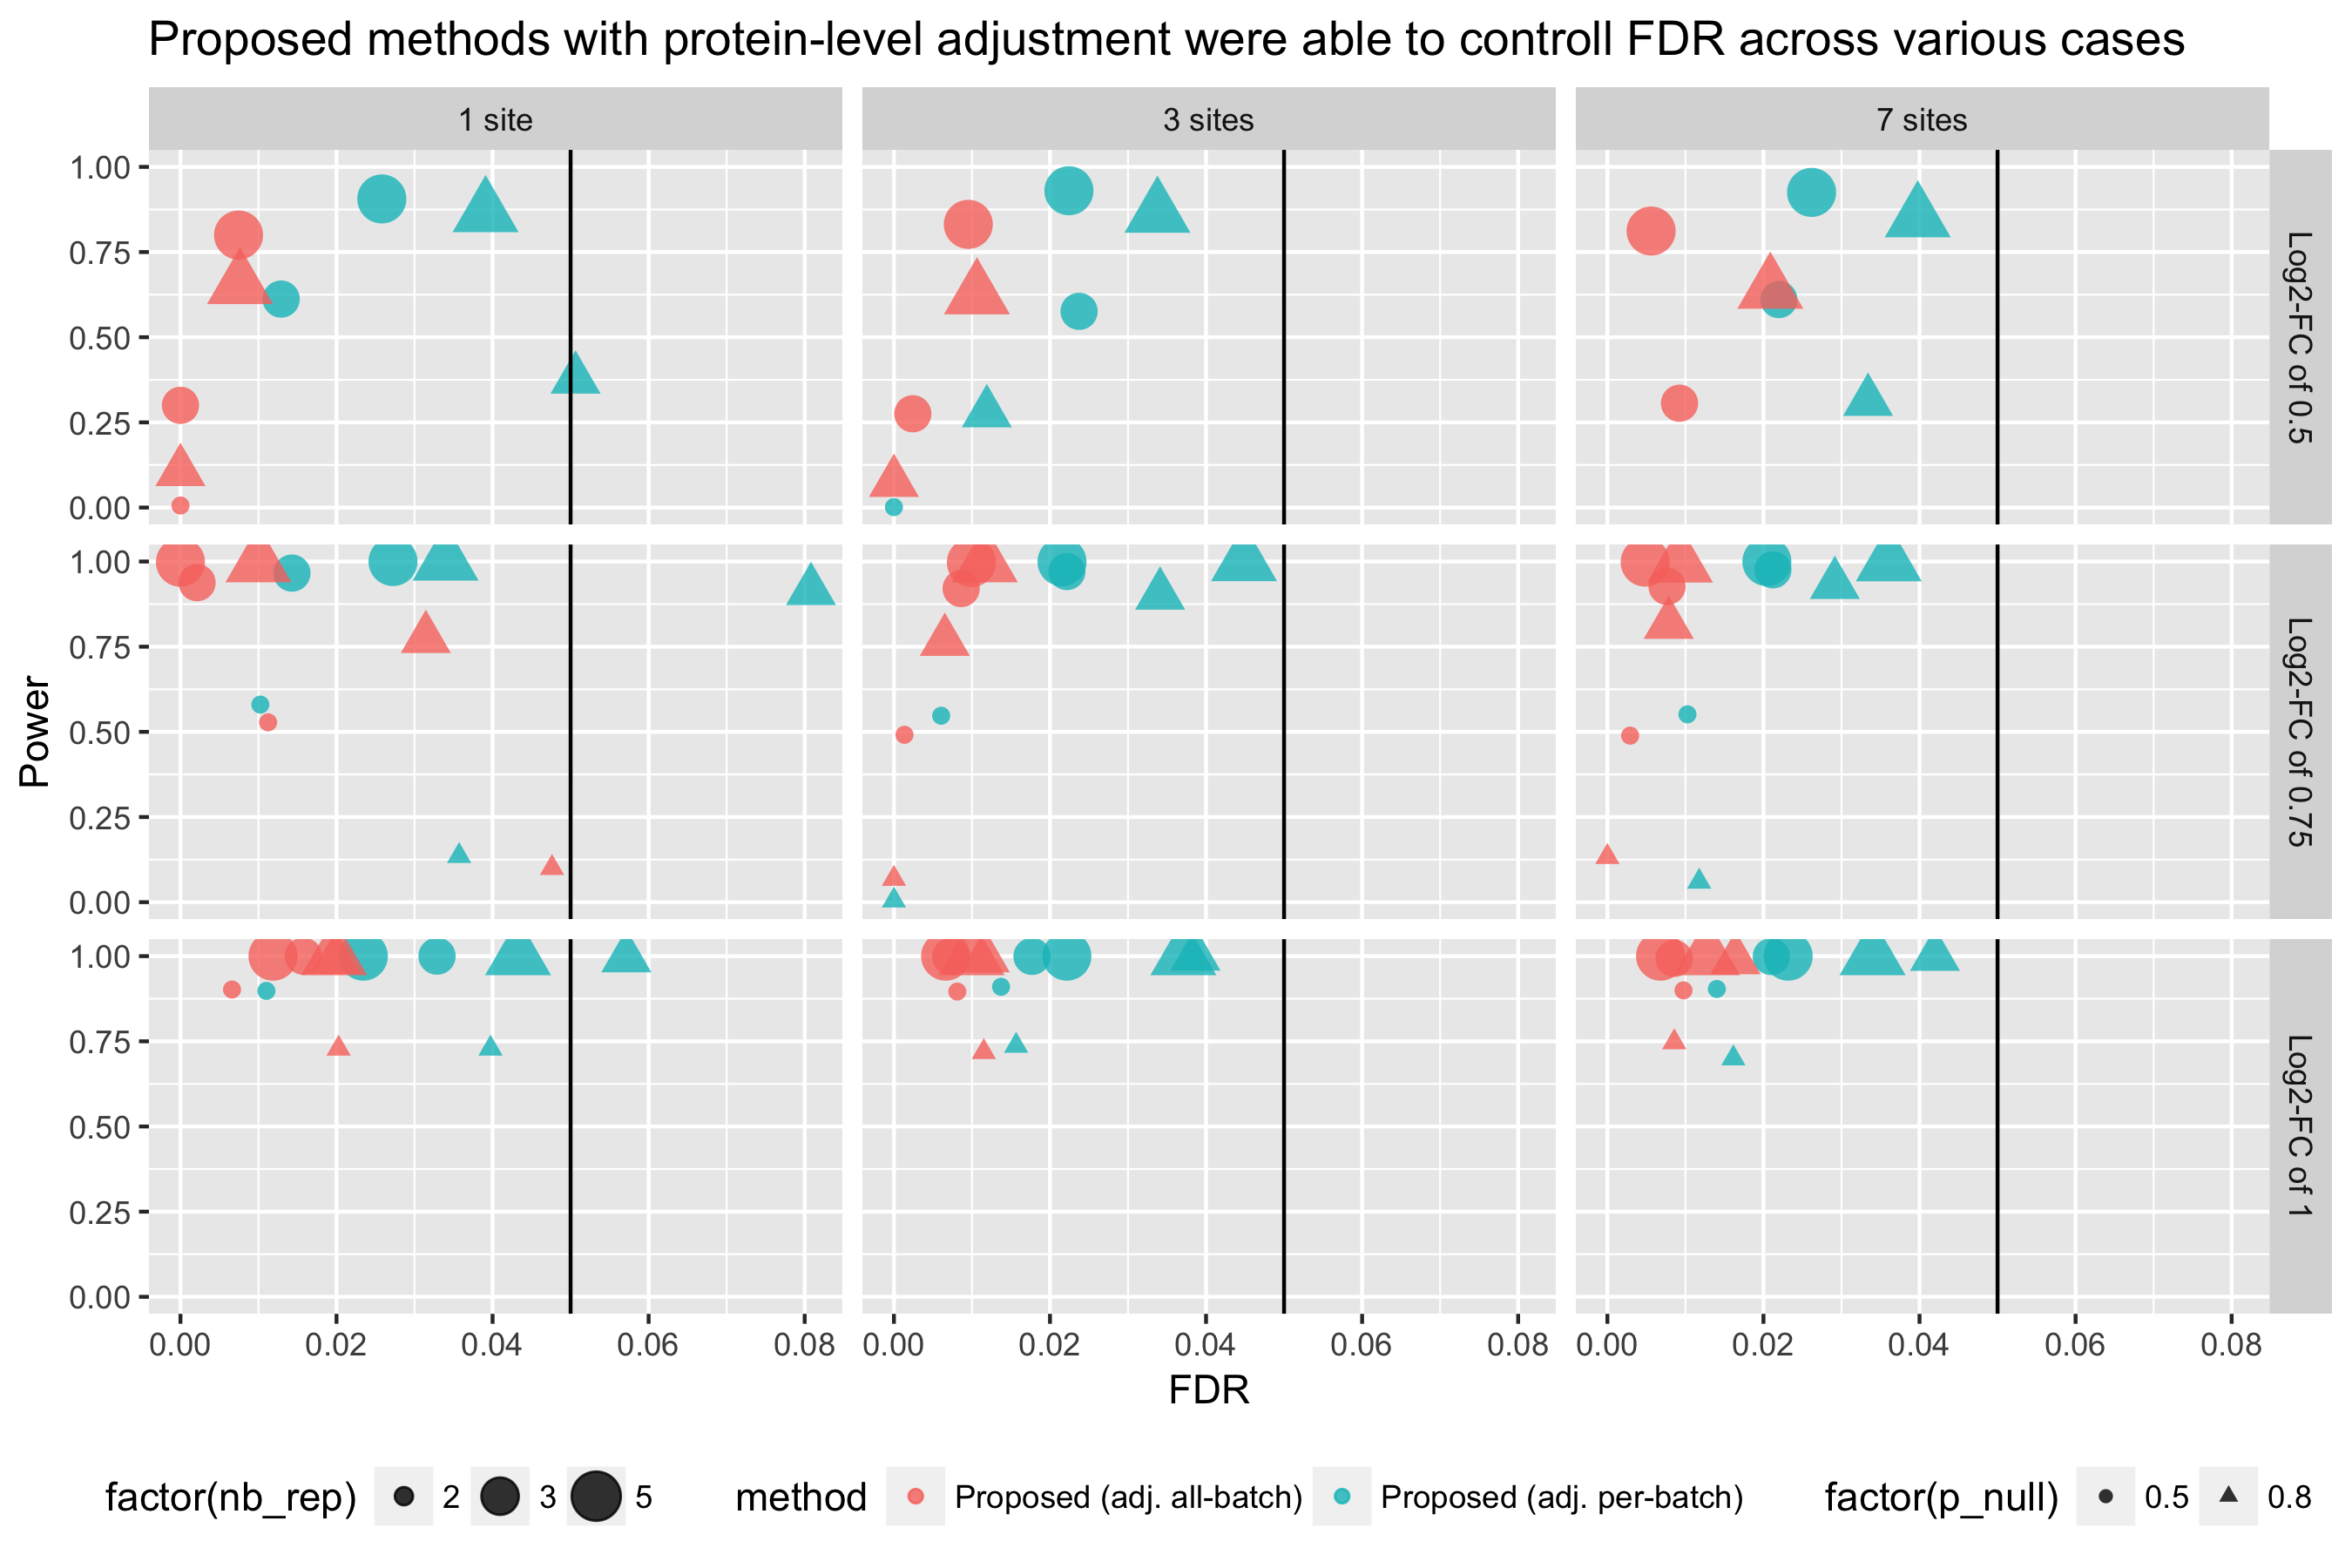
\includegraphics[width=.85\textwidth]{sim/prot_fdr}
\caption{Correlation between test statistics across sites due to protein-level adjustment did not affect the expected level of FDR under the considered scenarios. The Benjamini-Hochberg procedure was used to control the FDR. \label{fig:prot_fdr}}
\end{figure}

\todo{Storey's method?}
\todo{Proportion of null doesn't seem to be a big factor}


\clearpage
%%%%%%%%%%%%%%%%%%%%%%%%%%%%%%%%%%%%%%%%%%%%%%%%%%%%%%%%%%%%%%%%%
\section{Appendix}

This section contains full details of some plots that we are trying to simplify. It is only for the reference during the preparation and will be removed later. 


\end{document} 








%%%%%%%%%%%%%%%%%%%%%%%%%%%%%%%%%%%%%%%%%%%%%%%%%%%%%%%%%%%%%%%%%
%\section{Modeling and inference: one batch}
%
%
%%%%%%%%%%%%%%%%%%%%%%%%%%%%%%%%%%%%%%%%%%%%%%%%%%%%%%%%%%%%%%%%%
%\subsection{Linear models and parameter estimation}
%\paragraph{Model.}
%For a protein, the observed log-intensity of a modified peptide feature is denoted by $y_{ijk}^{\ast}$ and represented using a linear mixed model
%\[
%y_{ijk}^{\ast} = \psi^{\ast} + \text{Group}_{i}^{\ast} + \text{Run}_{j(i)}^{\ast} + \text{Feature}_{k}^{\ast} + (\text{Run} \times \text{Feature})_{ijk}^{\ast},
%\]
%\[
%i = 1, \ldots, I, \quad j = 1, \ldots, J, \quad k = 1, \ldots, K
%\]
%where $\psi^{\ast}$ is the expected value of log-abundance of the modification, and the effects of condition, run, and feature characterize how the log-intensity of each feature deviates from this reference. The interaction between run and feature $(\text{Run} \times \text{Feature})_{ijk}^{\ast}$ is essentially viewed as a random noise. The effects of condition and feature are modeled as fixed effects: 
%\[
%\sum_{i=1}^{I} \text{Group}_{i}^{\ast} = 0, \quad \sum_{k=1}^{K} \text{Feature}_{k}^{\ast} = 0,
%\]
%and the effects of run and its interaction with feature are considered as random effects arising from normal distribution with mean $0$: 
%\[
%\text{Run}_{j(i)}^{\ast} = \gamma_{j(i)}^{\ast} \stackrel{\text{iid}}{\sim} \mathcal{N}(0, \sigma_{\gamma^{\ast}}^{2}), \qquad 
%(\text{Run} \times \text{Feature})_{ijk}^{\ast} = \epsilon_{ijk}^{\ast} \stackrel{\text{iid}}{\sim} \mathcal{N}(0, \sigma_{\epsilon^{\ast}}^{2}).
%\]
%%\[
%%\text{Run}_{j(i)}^{\ast} = \gamma_{j(i)}^{\ast} \stackrel{\text{iid}}{\sim} \mathcal{N}(0, \sigma_{\gamma^{\ast}}^{2}),
%%\]
%%\[
%%(\text{Run} \times \text{Feature})_{ijk}^{\ast} = \epsilon_{ijk}^{\ast} \stackrel{\text{iid}}{\sim} \mathcal{N}(0, \sigma_{\epsilon^{\ast}}^{2}).
%%\]
%Similarly, the observed log-intensity of an unmodified peptide feature is denoted by $y_{ijk}$ and represented as 
%\[
%y_{ijl} = \psi + \text{Group}_{i} + \text{Run}_{j(i)} + \text{Feature}_{l} + (\text{Run} \times \text{Feature})_{ijl}, 
%\]
%where $\psi$ the expected value of log-abundance of the protein, the effects of condition and feature are modeled as fixed effects: 
%\[
%\sum_{i=1}^{I} \text{Group}_{i} = 0, \quad \sum_{l=1}^{L} \text{Feature}_{l} = 0,
%\]
%and 
%\[
%\text{Run}_{j(i)} = \gamma_{j(i)} \stackrel{\text{iid}}{\sim} \mathcal{N}(0, \sigma_{\gamma}^{2}), \qquad 
%(\text{Run} \times \text{Feature})_{ijl} = \epsilon_{ijl} \stackrel{\text{iid}}{\sim} \mathcal{N}(0, \sigma_{\epsilon}^{2}).
%\]
%
%\paragraph{Parameter estimation.} The parameter estimation is performed by using a sub-plot model to summarize feature intensities per run, followed by a whole-plot model to carry out the model-based inference of the underlying abundance. 
%
%\paragraph{Step 1 of parameter estimation: run-level summarization.} The sub-plot model is used for the summarization of feature intensities. This step involves 
%\begin{enumerate}
%\item Imputation of censored missing values
%\item Summarization of feature intensities using Tukey's median polish (TMP), where the summarized log-intensity is denoted by $\hat{y}_{ij}$
%\end{enumerate}
%
%\paragraph{Step 2 of parameter estimation: model-based inference of the underlying abundance.}
%The whole-plot model for the modification abundance in each run is represented as 
%\[
%\hat{y}_{ij}^{\ast} = \psi^{\ast} + \text{Group}_{i}^{\ast} + \text{Run}_{j(i)}^{\ast},
%\]
%where $\sum_{i=1}^{I} \text{Group}_{i}^{\ast} = 0$, $\text{Run}_{j(i)}^{\ast} = \gamma_{j(i)}^{\ast} \stackrel{\text{iid}}{\sim} \mathcal{N}(0, \sigma_{\gamma^{\ast}}^{2})$.
%Similarly, the model for protein abundance in each run is given by
%\[
%\hat{y}_{ij} = \psi + \text{Group}_{i} + \text{Run}_{j(i)},
%\]
%where $\sum_{i=1}^{I} \text{Group}_{i} = 0$, $\text{Run}_{j(i)} = \gamma_{j(i)} \stackrel{\text{iid}}{\sim} \mathcal{N}(0, \sigma_{\gamma}^{2})$. The expected values of log-abundances of the modification and protein in group $i$ are defined as $\mu_{i}^{\ast}$ and $\mu_{i}$, respectively. The values are represented as follows
%\begin{align*}
%\mu_{i}^{\ast} &= \psi^{\ast} + \text{Group}_{i}^{\ast} \\
%\mu_{i} &= \psi + \text{Group}_{i}.
%\end{align*}
%
%
%%%%%%%%%%%%%%%%%%%%%%%%%%%%%%%%%%%%%%%%%%%%%%%%%%%%%%%%%%%%%%%%%
%\subsection{Model-based inference}
%Hypothesis testing for differential modification.
%
%\paragraph{Hypothesis $H_{0}^{(1)}$.} The hypothesis states that there is no difference in log-abundance of the modification between groups $i$ and $i'$
%\begin{align*}
%H_{0}^{(1)}: \mu_{i}^{\ast} - \mu_{i'}^{\ast} &= 0 \\
%H_{a}^{(1)}: \mu_{i}^{\ast} - \mu_{i'}^{\ast} &\neq 0
%\end{align*}
%The estimated log of fold change in modification abundance is given by
%\[
%\hat{\mu}_{i}^{\ast} - \hat{\mu}_{i'}^{\ast} = \frac{1}{J} \left( \hat{y}_{i+}^{\ast} - \hat{y}_{i'+}^{\ast} \right),
%\]
%and the standard error of the estimate is 
%\[
%\mathrm{SE}\left( \hat{\mu}_{i}^{\ast} - \hat{\mu}_{i'}^{\ast} \right) = \sqrt{\frac{2}{J} \hat{\sigma}_{\gamma^{\ast}}^{2}}
%\]
%The test statistic $\left( \hat{\mu}_{i}^{\ast} - \hat{\mu}_{i'}^{\ast} \right) / \mathrm{SE}\left( \hat{\mu}_{i}^{\ast} - \hat{\mu}_{i'}^{\ast} \right)$ is compared against the $t$ distribution. The degrees of freedom of the $t$ distribution are $2J-2$.
%
%\paragraph{Hypothesis $H_{0}^{(2)}$.} The hypothesis states that there is no difference in log-abundance of the modification between groups $i$ and $i'$, normalized by the protein abundance 
%\begin{align*}
%H_{0}^{(2)}: \left( \mu_{i}^{\ast} - \mu_{i'}^{\ast} \right) - \left( \mu_{i} - \mu_{i'} \right) &= 0 \\
%H_{a}^{(2)}: \left( \mu_{i}^{\ast} - \mu_{i'}^{\ast} \right) - \left( \mu_{i} - \mu_{i'} \right) &\neq 0
%\end{align*}
%The estimated log of fold change in normalized modification abundance is given by
%\[
%\left( \hat{\mu}_{i}^{\ast} - \hat{\mu}_{i'}^{\ast} \right) - \left( \hat{\mu}_{i} - \hat{\mu}_{i'} \right) 
%= \frac{1}{J} \left( \hat{y}_{i+}^{\ast} - \hat{y}_{i'+}^{\ast} \right) - \frac{1}{J} \left( \hat{y}_{i+} - \hat{y}_{i'+} \right),
%\]
%and the standard error of the estimate is 
%\[
%\sqrt{\frac{2}{J} \left( \hat{\sigma}_{\gamma^{\ast}}^{2} + \hat{\sigma}_{\gamma}^{2} \right) }
%\]
%The test statistic is compared against the $t$ distribution with degrees of freedom approximated as:
%\[
%df = 
%\frac{ 2 (J-1) \left( \hat{\sigma}_{\gamma^{\ast}}^{2} + \hat{\sigma}_{\gamma}^{2} \right)^2 }{ \left( \hat{\sigma}_{\gamma^{\ast}}^{4} + \hat{\sigma}_{\gamma}^{4} \right) }.
%\]

%\paragraph{Hypothesis $H_{0}^{(1)}$.} The hypothesis states that there is no difference in log-abundance of the modification between groups $i$ and $i'$
%\begin{align*}
%H_{0}^{(1)}: \mu_{i}^{\ast} - \mu_{i'}^{\ast} &= 0 \\
%H_{a}^{(1)}: \mu_{i}^{\ast} - \mu_{i'}^{\ast} &\neq 0
%\end{align*}
%The log of fold change in modification abundance is estimated as the average over batches
%\[
%\hat{\mu}_{i}^{\ast} - \hat{\mu}_{i'}^{\ast} = 
%\frac{1}{B} \sum_{b=1}^{B} \left[ \frac{1}{J} \left( \hat{y}_{b,i+}^{\ast} - \hat{y}_{b,i'+}^{\ast} \right) \right],
%\]
%and the standard error of the estimate is 
%\[
%\mathrm{SE}\left( \hat{\mu}_{i}^{\ast} - \hat{\mu}_{i'}^{\ast} \right) = 
%\left[ \left(\frac{1}{B}\right)^2 \cdot \frac{2}{J} \sum_{b=1}^{B} \hat{\sigma}_{\gamma_b^{\ast}}^{2} \right]^{1/2}
%\]
%The test statistic $\left( \hat{\mu}_{i}^{\ast} - \hat{\mu}_{i'}^{\ast} \right) / \mathrm{SE}\left( \hat{\mu}_{i}^{\ast} - \hat{\mu}_{i'}^{\ast} \right)$ is compared against the $t$ distribution. The degrees of freedom of the $t$ distribution are approximated as
%\[
%\frac{ \left( \sum_{b=1}^{B} \hat{\sigma}_{\gamma_{b}^{\ast}}^{2} \right)^2 }
%%{ \sum_{b=1}^{B} \left( \hat{\sigma}_{\gamma_{b}^{\ast}}^{4} /  \mathrm{df}(\gamma_b^{\ast}) \right) }
%{ \sum_{b=1}^{B} \left[  \frac{\hat{\sigma}_{\gamma_{b}^{\ast}}^{4}}{ \mathrm{df}(\gamma_b^{\ast}) }  \right] }
%\]
%

%%%%%%%%%%%%%%%%%%%%%%%%%%%%%%%%%%%%%%%%%%%%%%%%%%%%%%%%%%%%%%%%
%\subsection{All-batch model}
%
%\paragraph{Step 1 of parameter estimation: run-level summarization.} As in the per-batch model.
%
%\paragraph{Step 2 of parameter estimation: model-based inference of the underlying abundance.}
%The whole-plot model for the modification abundance in each run is represented as 
%\[
%\hat{y}_{b, ij}^{\ast} = \psi^{\ast} + \delta_{b}^{\ast} + C_{i}^{\ast} + R_{b, j(i)}^{\ast},
%\]
%where $\sum_{b=1}^{B} \delta_{b}^{\ast} = 0$, $\sum_{i=1}^{I} C_{i}^{\ast} = 0$, $R_{b, j(i)}^{\ast} = \gamma_{b, j(i)}^{\ast} \stackrel{\text{iid}}{\sim} \mathcal{N}(0, \sigma_{\gamma^{\ast}}^{2})$.
%Similarly, the model for protein abundance in each run is given by
%\[
%\hat{y}_{b, ij} = \psi + \delta_{b} + C_{i} + R_{b, j(i)},
%\]
%where $\sum_{b=1}^{B} \delta_{b} = 0$, $\sum_{i=1}^{I} C_{i} = 0$, $R_{b, j(i)} = \gamma_{b, j(i)} \stackrel{\text{iid}}{\sim} \mathcal{N}(0, \sigma_{\gamma}^{2})$. The expected values of log-abundances of the modification and protein in group $i$ are defined as $\mu_{i}^{\ast}$ and $\mu_{i}$, respectively. The values are represented as follows
%\begin{align*}
%\mu_{i}^{\ast} &= \psi^{\ast} + C_{i}^{\ast}\\
%\mu_{i} &= \psi + C_{i}
%\end{align*}
